%%%%%%%%%%%%%%%%%%%%%%%%%%%%%%%%%%%%%%%%%%%%%%%%%%%%%%%%%%%%%%%%%%%%%%%%%%%%%%%%
% event_selection.tex: 
%%%%%%%%%%%%%%%%%%%%%%%%%%%%%%%%%%%%%%%%%%%%%%%%%%%%%%%%%%%%%%%%%%%%%%%%%%%%%%%%
\chapter{Event Selection}
\label{sec:event_selection_chapter}
%%%%%%%%%%%%%%%%%%%%%%%%%%%%%%%%%%%%%%%%%%%%%%%%%%%%%%%%%%%%%%%%%%%%%%%%%%%%%%%%

The LRS model predicts the existence of a \WR and \nul that decay to two charged leptons and two jets, all with 
high transverse energy.  Using the 2.6 fb$^{-1}$ \cite{lumi} of data recorded by CMS from September through November 
2015, evidence of a \WR and \nul was searched for as an excess of events in data with $eejj$ and $\mu\mu jj$ final 
states above the predicted backgrounds - \DY, \ttbar, W+jets, diboson processes, and QCD - and their uncertainties.  
The selections applied to data events were developed based on differences in lepton and jet kinematic distributions 
between \WR signal and background events.


\section{Selections based on \WR signal and ST backgrounds}
\label{sec:signalAndBkgndFeatures}
The event selections were driven by model independent features of \WR and \nul decays, and ST backgrounds in the $\ell\ell jj$ 
final states.  The expected \WR mass (\mWR) is large, above 2 $\TeV$, relative to the 13 $\TeV$ collision energy, 
so \WR bosons are expected to have low net momentum.  Therefore, the charged lepton and jet decay products, on average, 
are distributed uniformly in $\phi$, and are concentrated in the $|\eta| < 2.4$ region\footnote{The $|\eta| < 2.4$ region 
covers 94\% of the $0 \leq \theta < 180$ degree phase space, where $\theta = 0$ points along the beam axis.}, 
as shown in Figures \ref{fig:wrLeptonEtas} and \ref{fig:wrJetEtas}.  Furthermore, the large expected \mWR means final 
state leptons and jets should have $\pt$ of several hundred $\GeV$ or more, as shown in Figures \ref{fig:wrLeptonPts} and 
\ref{fig:wrJetPts}.  In contrast, the ST backgrounds in the $\ell\ell jj$ final states produce leptons and jets primarily 
with $\pt < 100$ $\GeV$, as shown in Figures \ref{fig:bkgLeptonPts} and \ref{fig:bkgJetPts}.  These differences in 
lepton and jet kinematics between signal and background events motivated the following event selections:

\begin{itemize}
	\item Two leptons were reconstructed with $\pt > 53$ $\GeV$, and one with $\pt > 60$ $\GeV$.
	\item Two jets were reconstructed with $\pt > 40$ $\GeV$.
	\item Both leptons and jets were reconstructed with $|\eta| < 2.4$.
	\item The invariant mass $\Mlljj$ of the reconstructed leptons and jets exceeded $\Mlljj > 600$ $\GeV$.
\end{itemize}

The \WR decays to a ST charged lepton $\ell$ (mass $m_{\ell}$) and a \nul (mass \mnul), and the large expected difference 
between their masses $m_{\ell}$ and \mnul motivated additional event selections.  As \mnul decreases towards the $Z$ boson 
mass, mixing between left- and right-handed neutrinos increases, and producing events with a ST neutrino and a charged lepton 
through $pp \rightarrow Z \rightarrow \nu\nu \rightarrow \nul\nu,\quad \nul \rightarrow \ell\WR^{*}$ becomes more likely.  
Evidence of \nul production through this process has not been found in Run I or II data \cite{gammaZinvisResult,higgsInvisResultsRunIandII}, 
so \mnul is expected to exceed the $Z$ boson mass, and thus $m_{\ell}$.  Due to this mass difference, the charged 
lepton $\ell_{1}$ from $\WR \rightarrow \nul\ell_{1}$ recoils against the heavier \nul to conserve momentum.  Then, 
the \nul decays to a second lepton $\ell_{2}$ and a dijet system $jj$, which recoil against each other.  As long as the \nul 
momentum is not $\gtrsim$10$\times \mnul$, the recoil between the dijet system and $\ell_{2}$, on average, produces a 
$\Delta R > 0.4$ separation between $\ell_{2}$ and both jets.  In addition, since $m_{\ell}$ is much less than \mnul and \mWR, 
$\ell_{2}$ ($\ell_{1}$) is equally likely to be emitted in any direction relative to the \nul (\WR) momentum.  Therefore, in 
approximately half of all \WR decays the angular separation between $\ell_{1}$ and $\ell_{2}$ in a plane that contains both of 
their momentum vectors is greater than $\frac{\pi}{2}$, which means the dilepton mass $\Mll$ is greater than $\sqrt{2} p_{1}p_{2}$, 
where $p_{i}$ is the momentum magnitude of $\ell_{i}$.  The final state leptons and jets are essentially massless with 
respect to the \WR, so on average the lepton momentum magnitude sum is $p_{1} + p_{2} = \mWR / 2$, and the geometric mean of 
lepton momentum magnitudes is $\mWR / \sqrt{8}$.  Thus, in approximately half of all \WR decays $\Mll$ is greater than $\mWR /2$.  
In contrast, the two dominant backgrounds - \ttbar and \DY - produce more than 50\% of their $\ell\ell jj$ events with 
$\Mll < 200$ $\GeV$, several hundred $\GeV$ below $\mWR / 2$ for the majority of signal mass hypotheses tested in the search 
presented in this thesis.  In addition, in QCD multijet and W+jets background events where two leptons were reconstructed, 
at least one lepton was often a byproduct of hadronization, and was reconstructed near but not clustered into a jet.  These 
differences between the signal and ST backgrounds in the $\Mll$ and $\Delta R(\ell,j)$ variables motivated the following 
additional event selections:

\begin{itemize}
	\item Each reconstructed lepton was separated from the other lepton and both jets by $\Delta R > 0.4$.
	\item The dilepton mass $\Mll$ of the two reconstructed leptons exceeded $\Mll > 200$ $\GeV$.
\end{itemize}


\begin{figure}[btp]
	\centering
	\subfigure{
		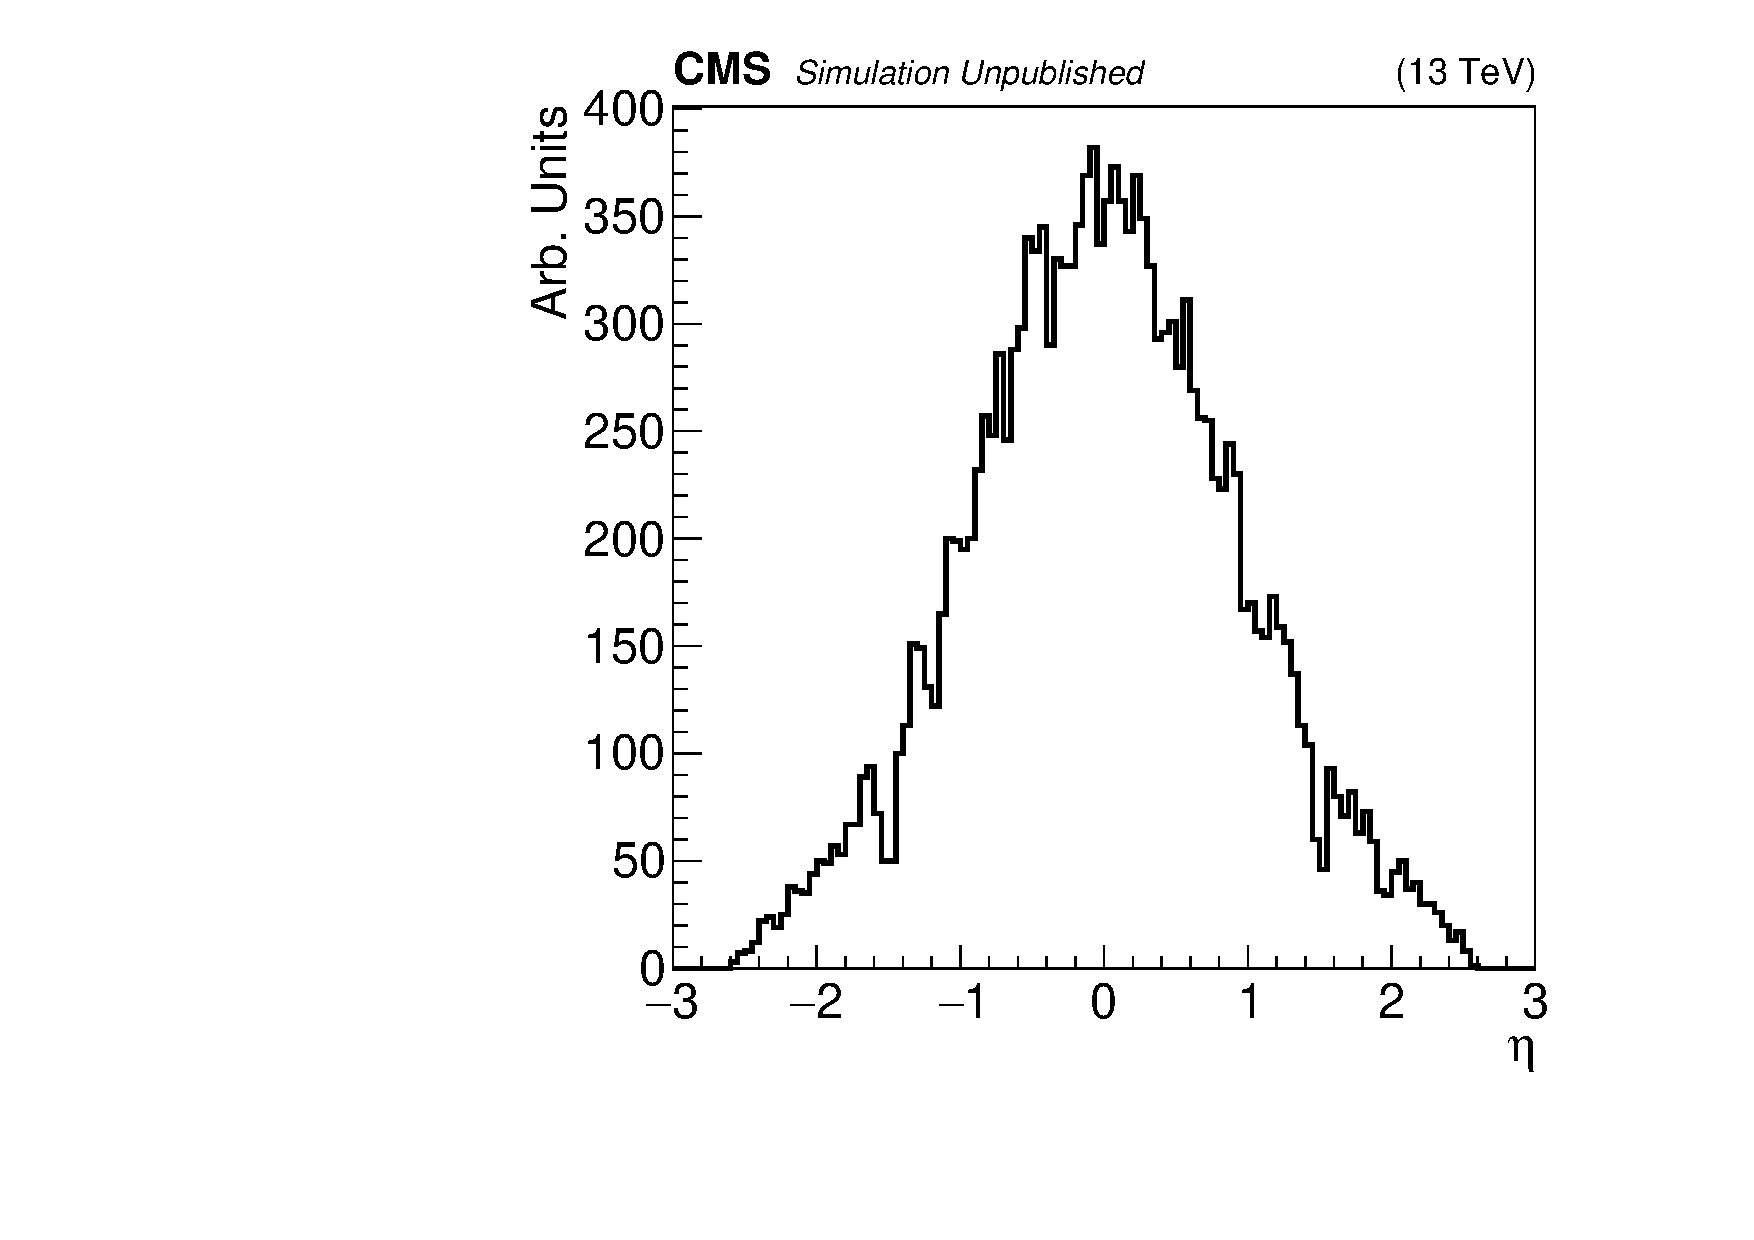
\includegraphics[width=0.45\textwidth]{figures/etaMatchedRecoEleFromWr_mwr2200_mnu1100.pdf}
	}
	\subfigure{
		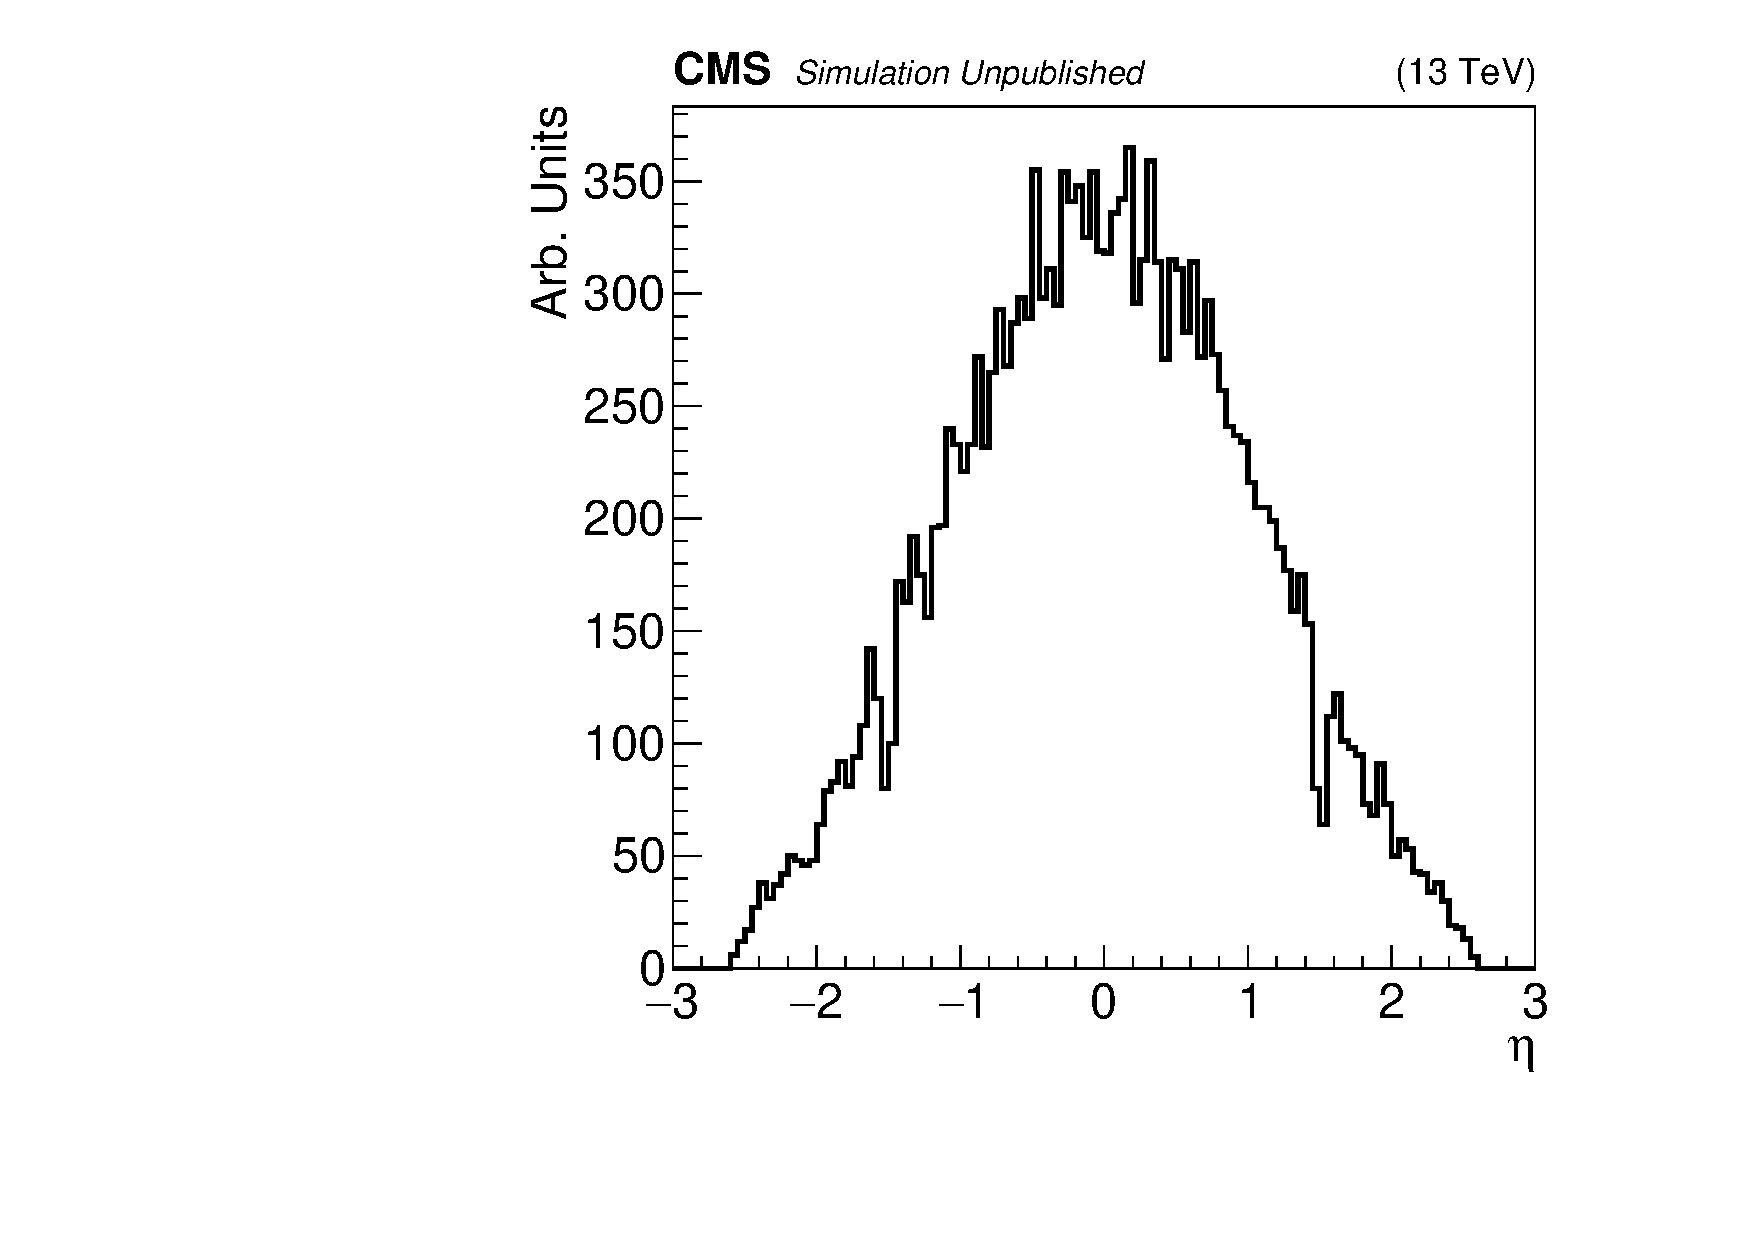
\includegraphics[width=0.45\textwidth]{figures/etaMatchedRecoEleFromNu_mwr2200_mnu1100.pdf}
	}
	\label{fig:wrLeptonEtas}
	\caption{The $\eta$ distribution of the reconstructed electron produced by the \WR (\nul) decay is shown on the top (bottom) for 
		simulated $\WR \rightarrow eejj$ events with $\mWR = 2.2 \TeV$ and $\mnul = 1.1 \TeV$.}
\end{figure}

\begin{figure}[btp]
	\centering
	\subfigure{
		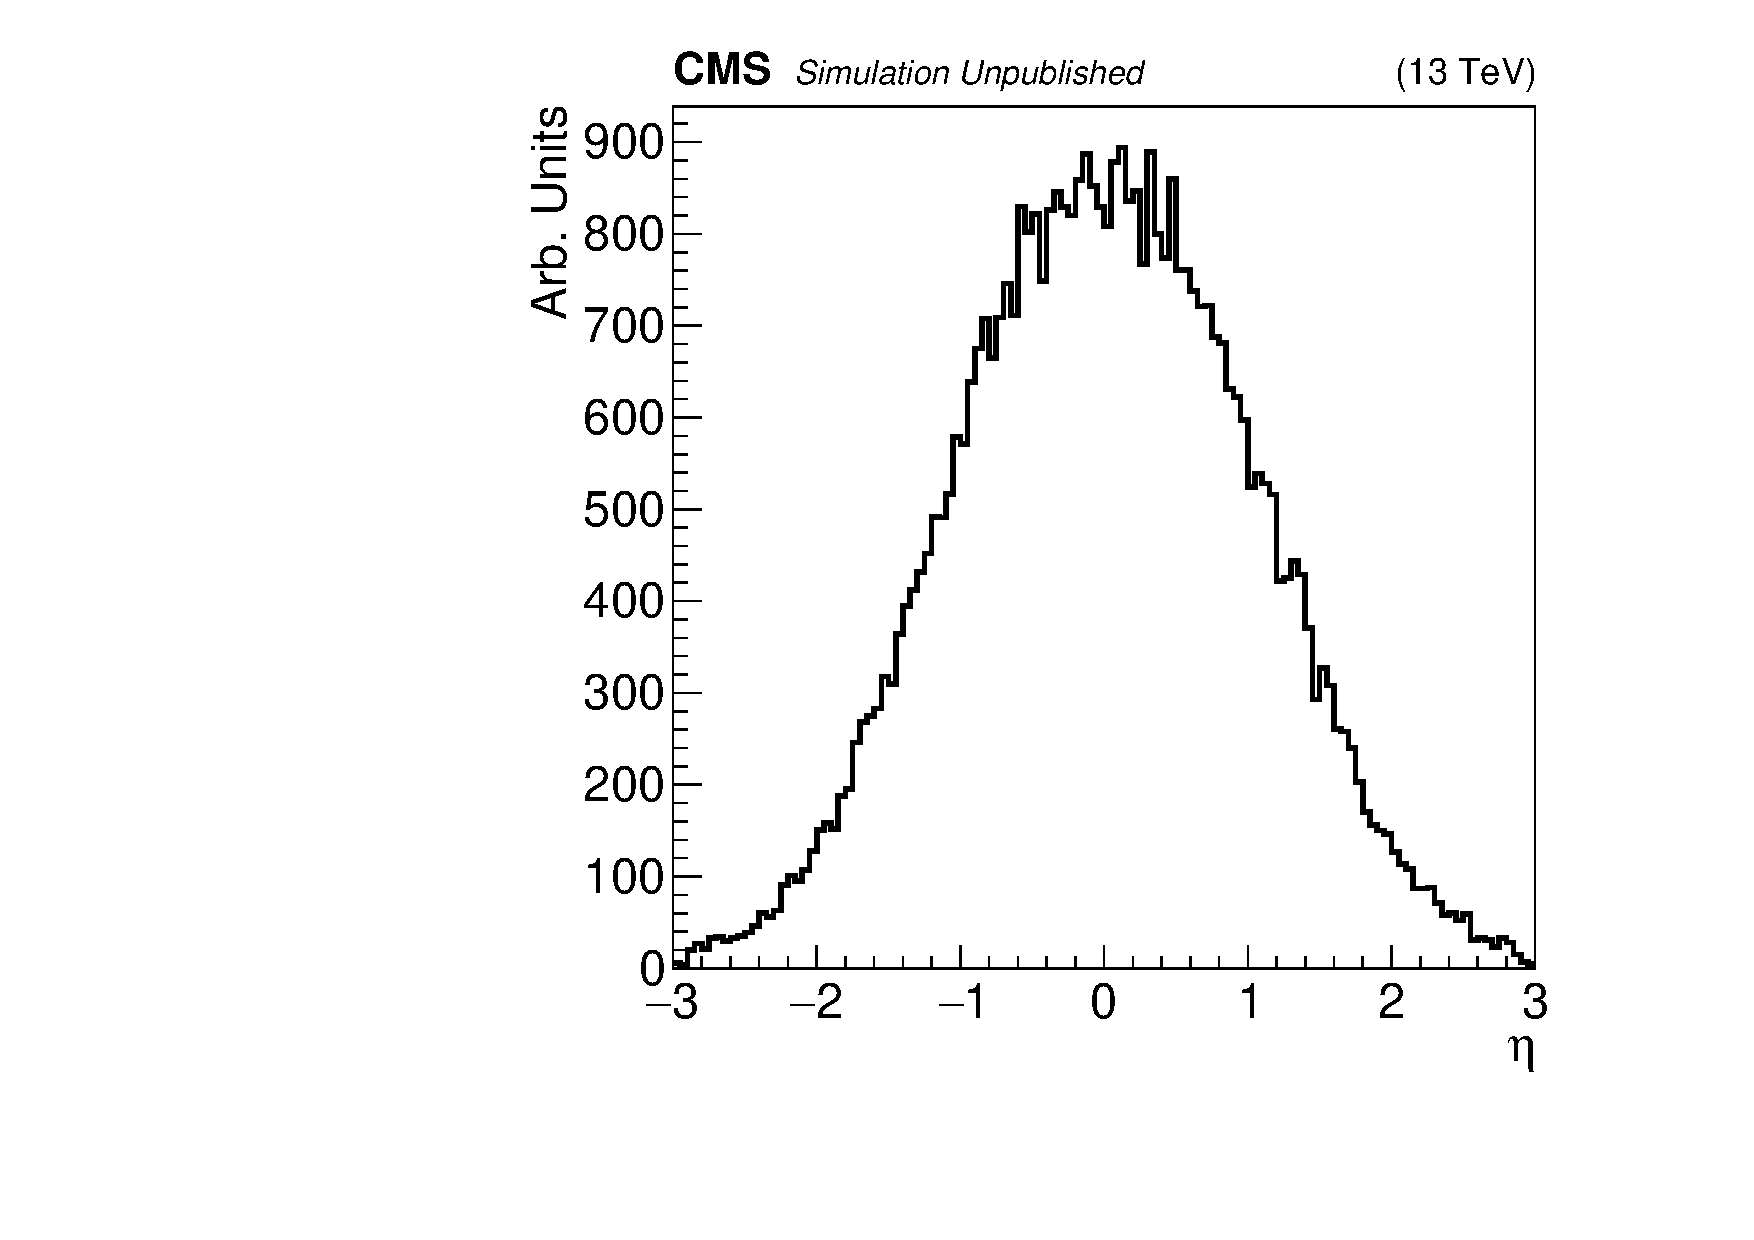
\includegraphics[width=0.45\textwidth]{figures/etaMatchedRecoJetOne_mwr2200_mnu1100.pdf}
	}
	\subfigure{
		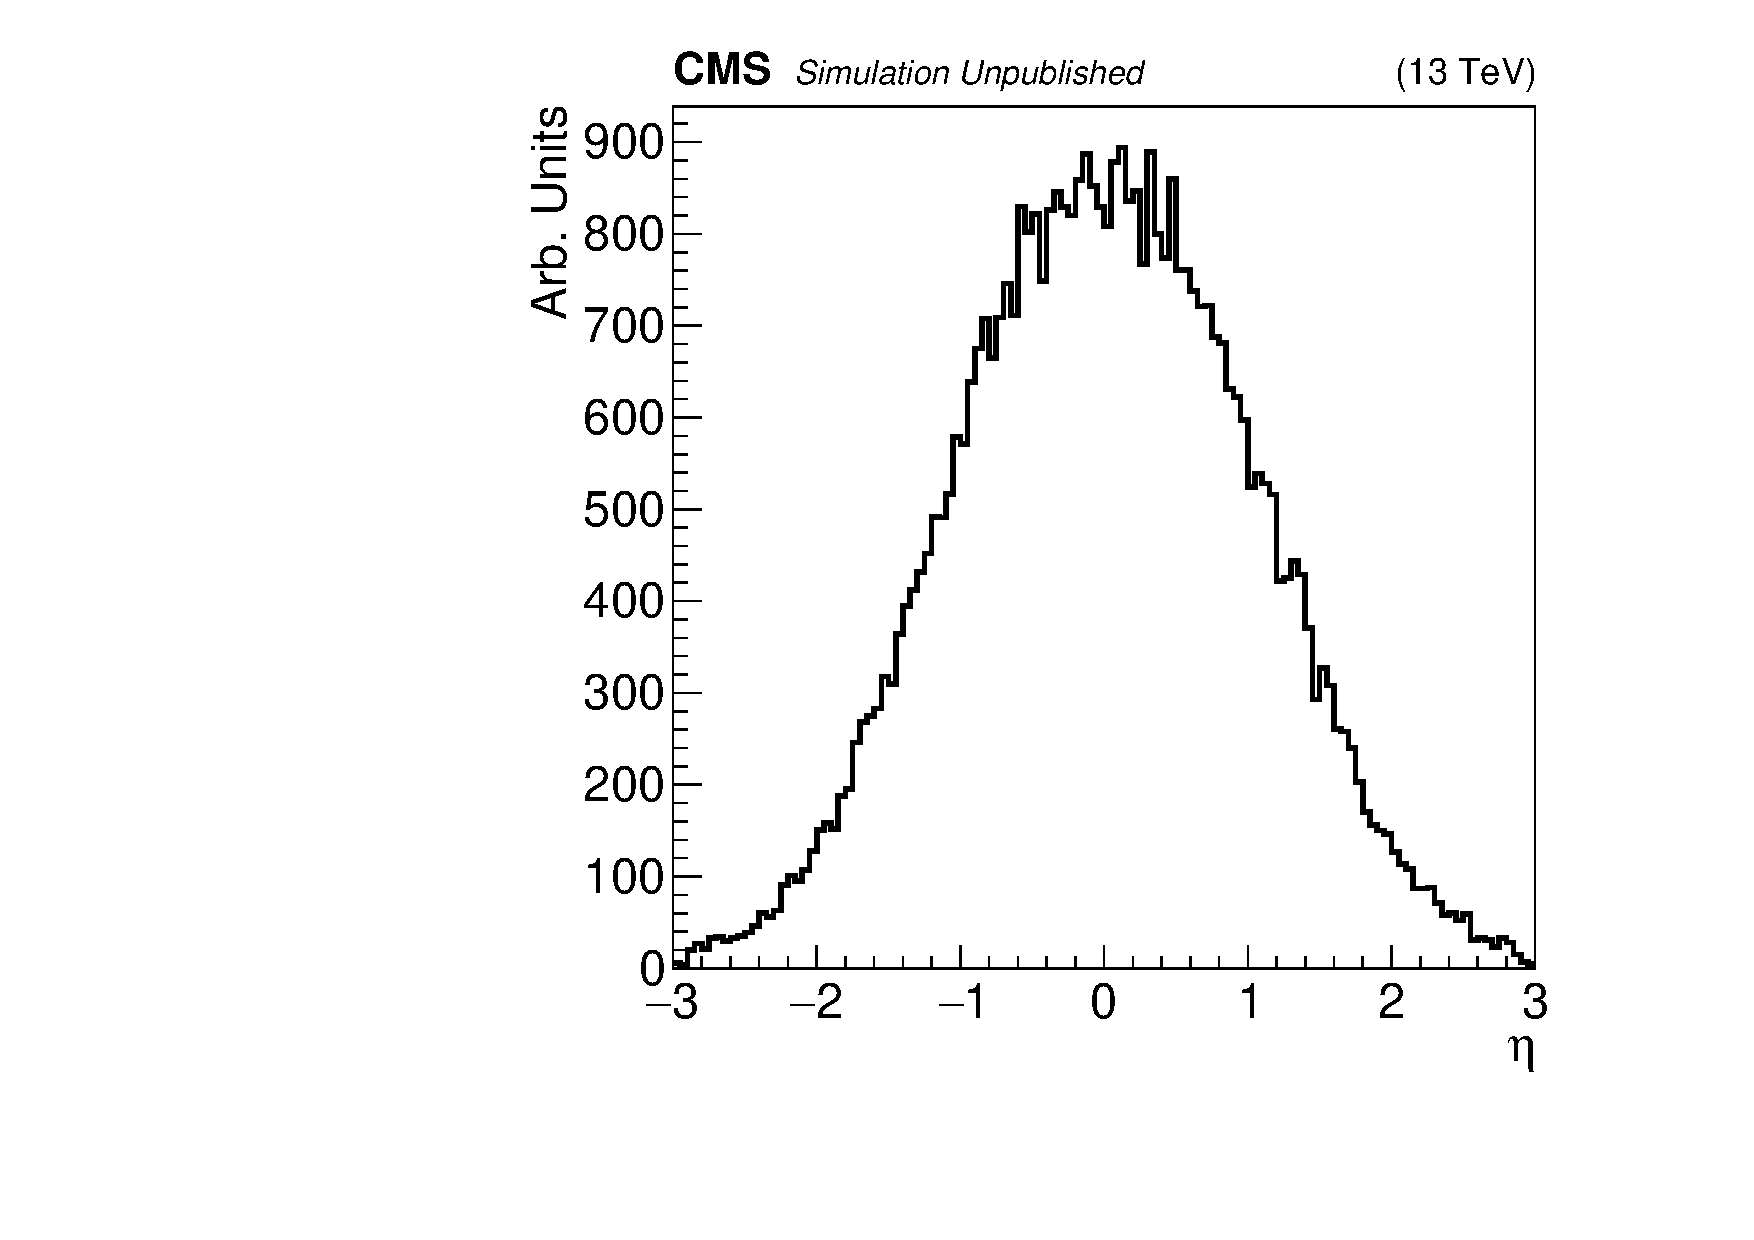
\includegraphics[width=0.45\textwidth]{figures/etaMatchedRecoJetOne_mwr2200_mnu1100.pdf}
	}
	\label{fig:wrJetEtas}
	\caption{The $\eta$ distributions of the reconstructed jets produced by the \nul decay are shown for 
		simulated $\WR \rightarrow eejj$ events with $\mWR = 2.2 \TeV$ and $\mnul = 1.1 \TeV$.}
\end{figure}

\begin{figure}[btp]
	\centering
	\subfigure{
		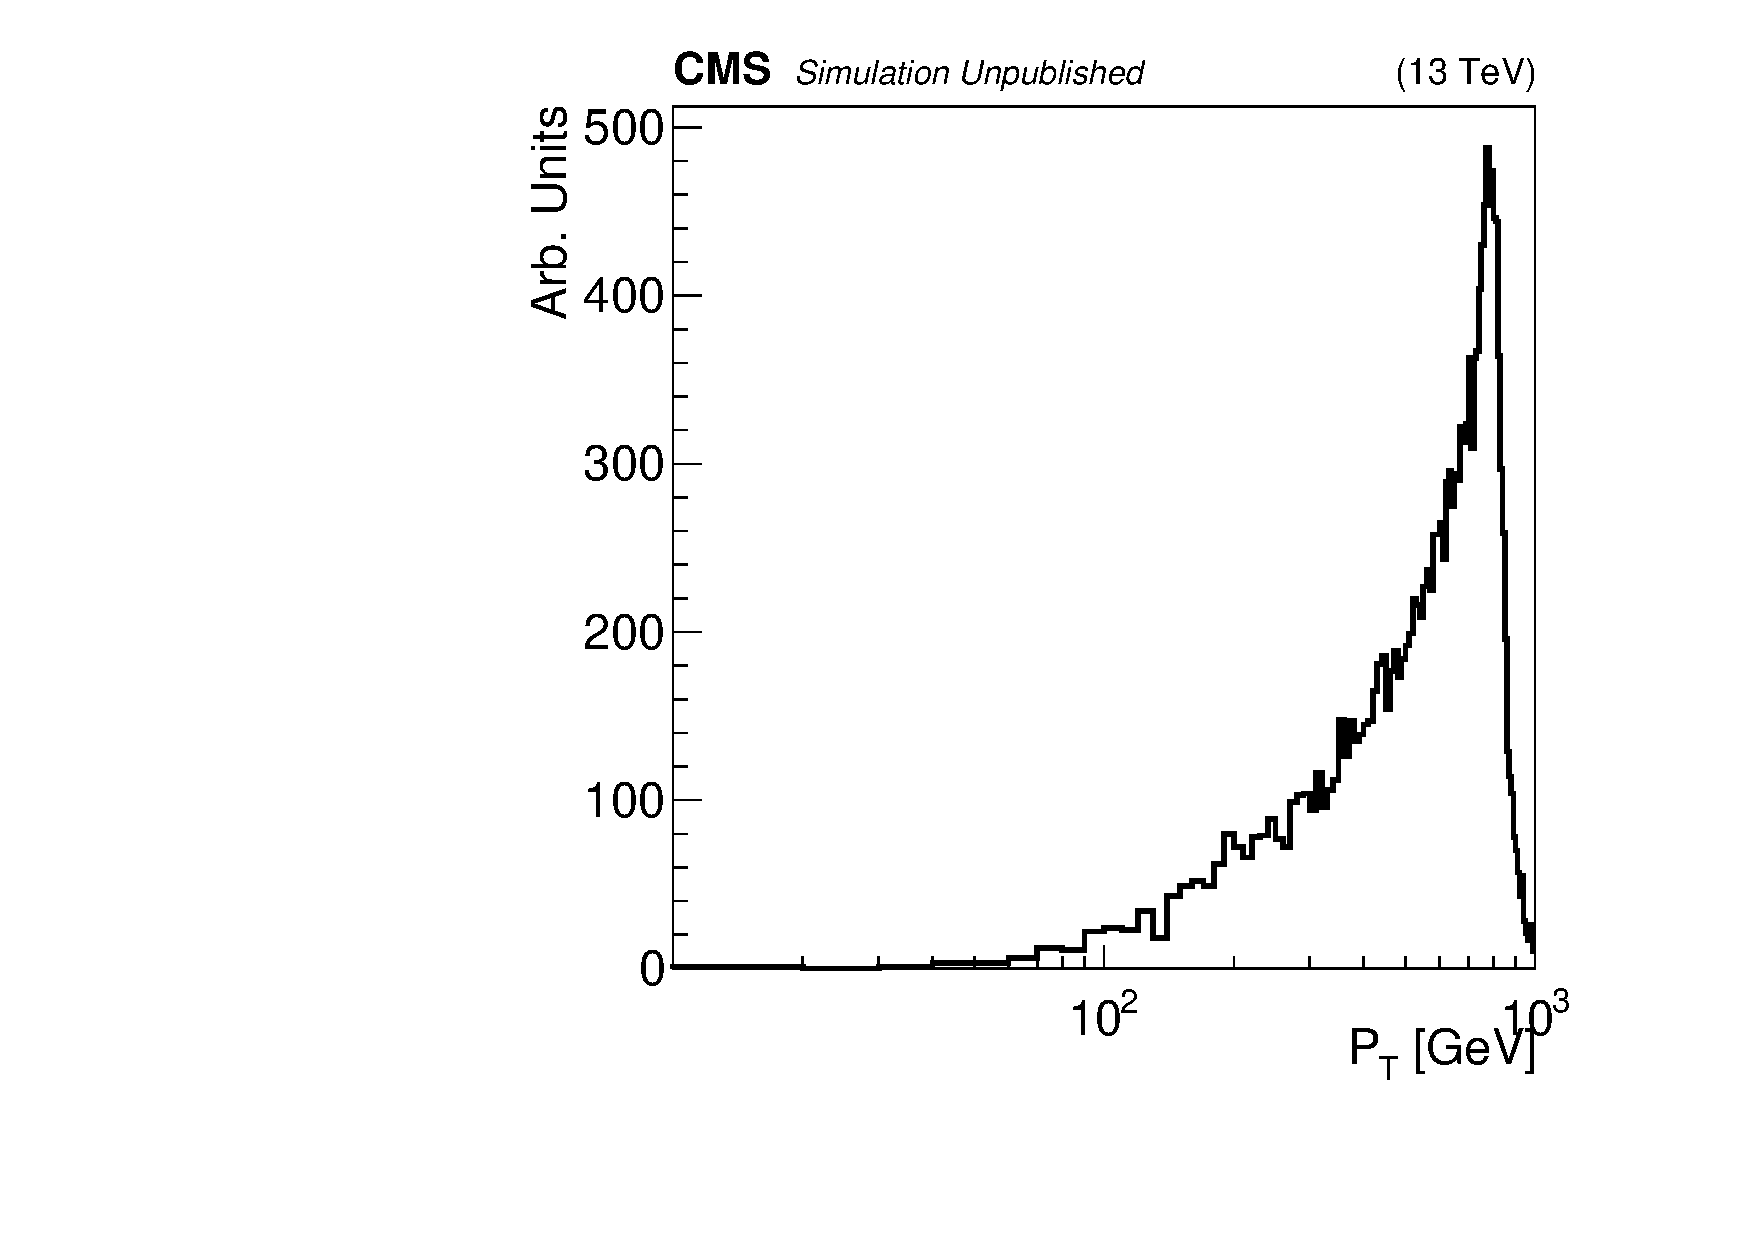
\includegraphics[width=0.45\textwidth]{figures/ptMatchedRecoEleFromWr_mwr2200_mnu1100.pdf}
	}
	\subfigure{
		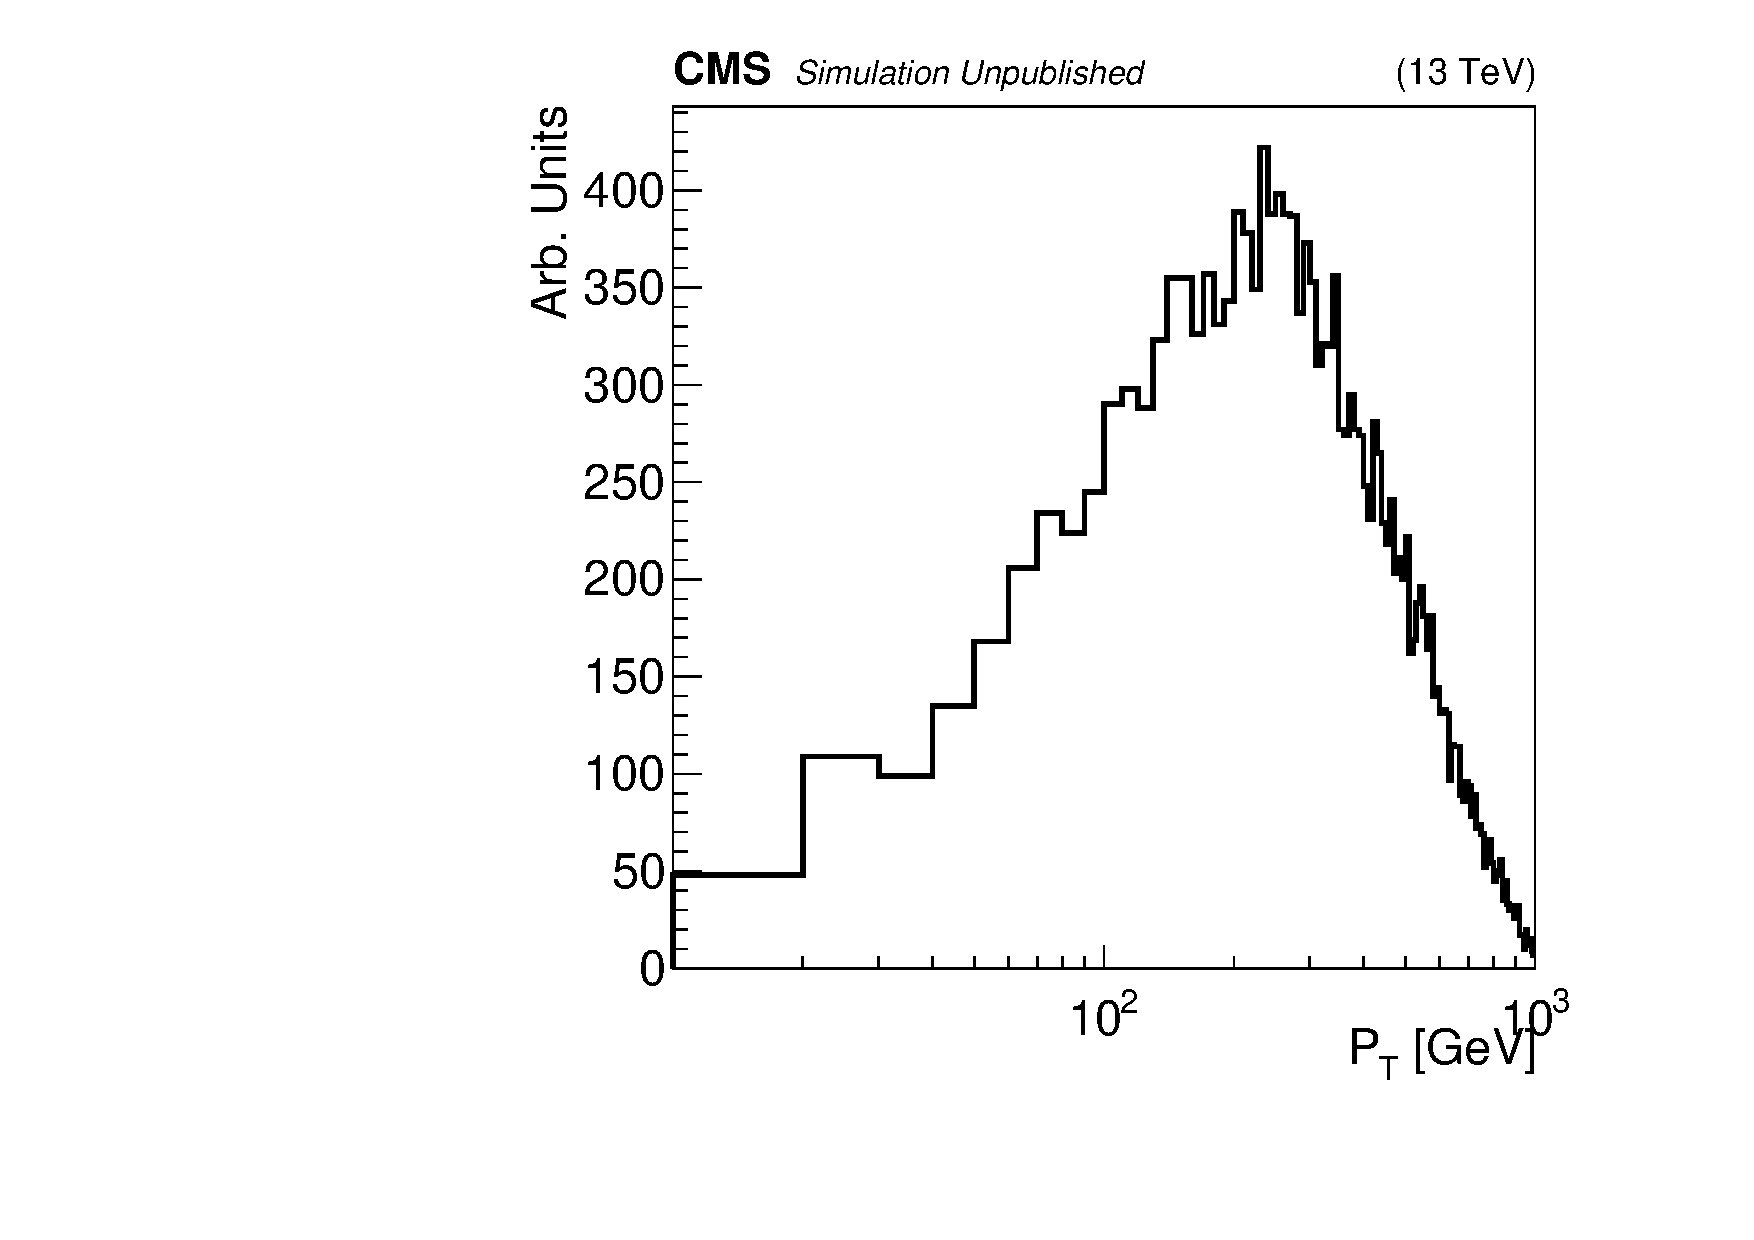
\includegraphics[width=0.45\textwidth]{figures/ptMatchedRecoEleFromNu_mwr2200_mnu1100.pdf}
	}
	\label{fig:wrLeptonPts}
	\caption{The $\pt$ distribution of the reconstructed electron produced by the \WR (\nul) decay is shown on the top (bottom) for 
		simulated $\WR \rightarrow eejj$ events with $\mWR = 2.2 \TeV$ and $\mnul = 1.1 \TeV$.}
\end{figure}

\begin{figure}[btp]
	\centering
	\subfigure{
		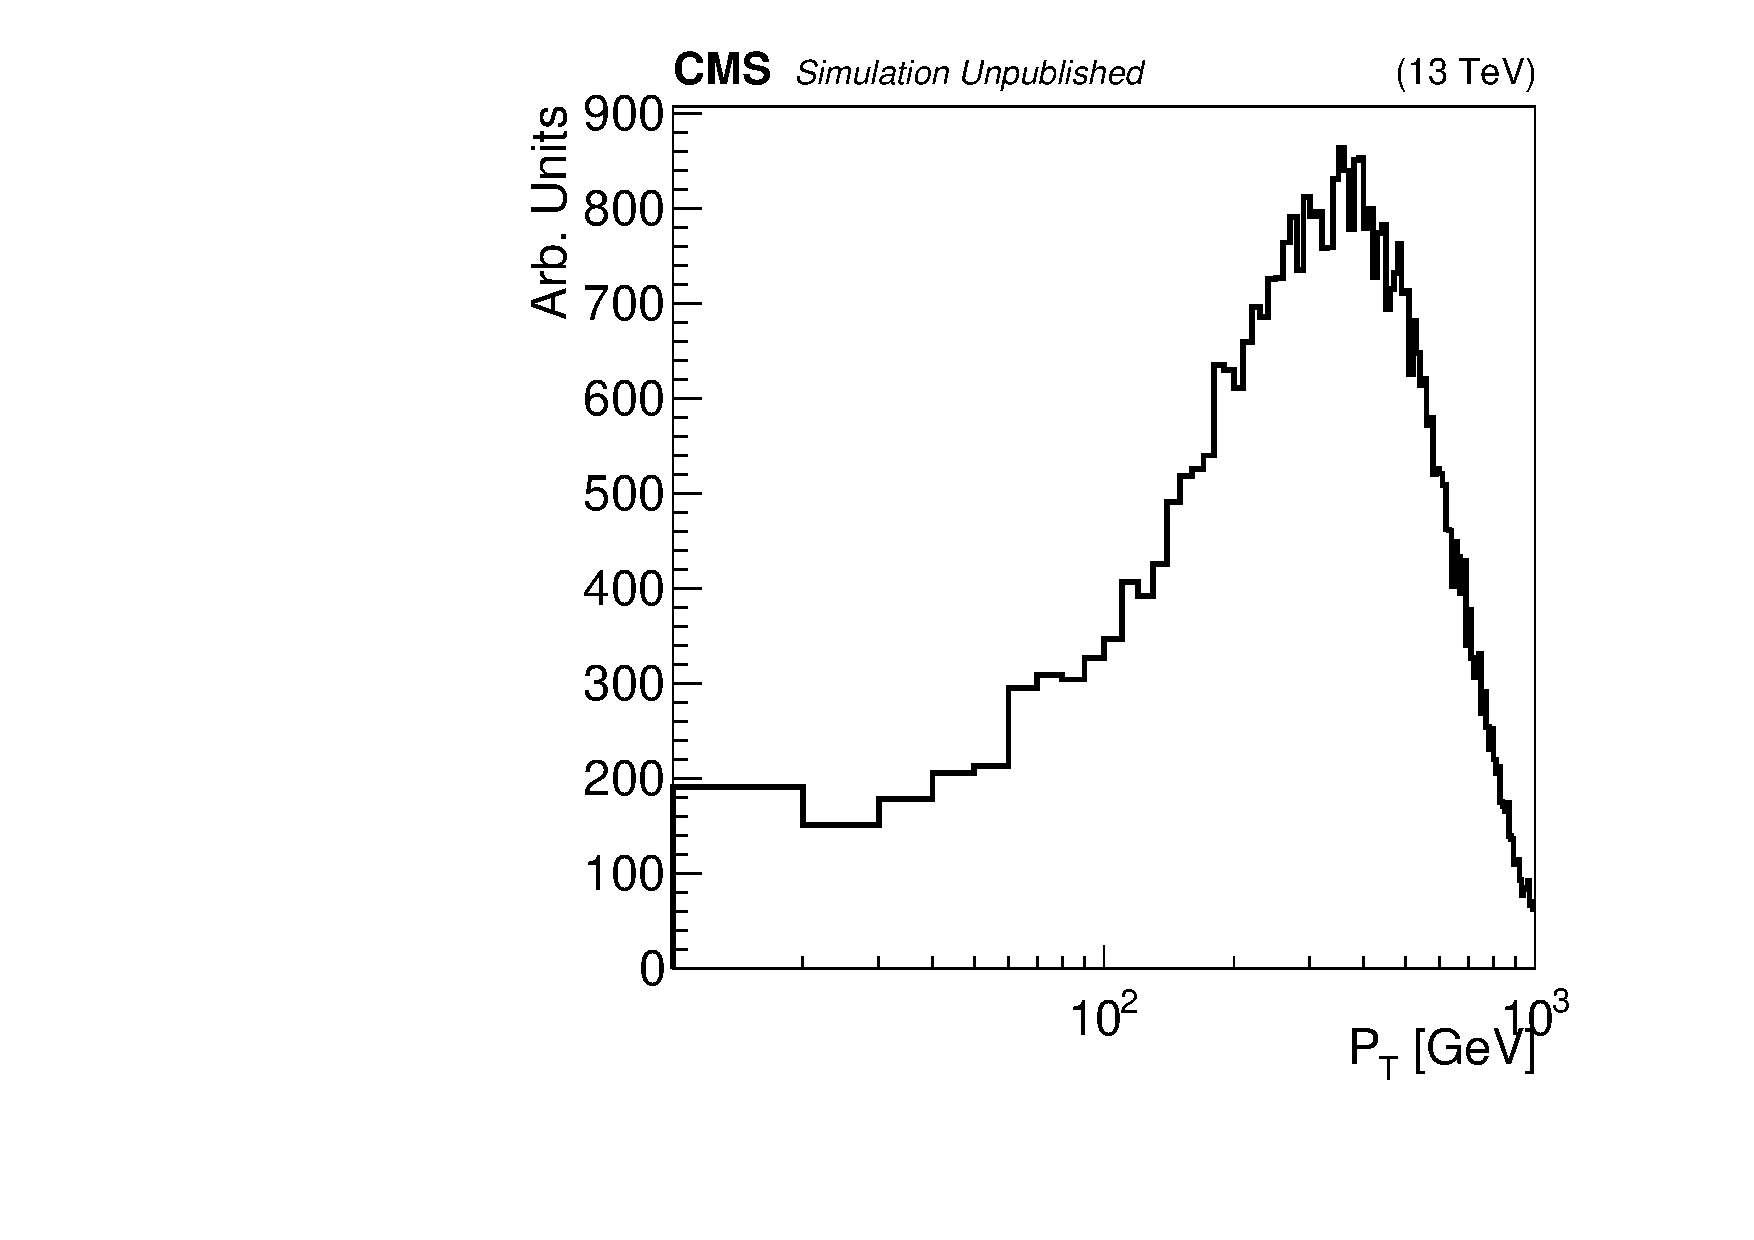
\includegraphics[width=0.45\textwidth]{figures/ptMatchedRecoJetOne_mwr2200_mnu1100.pdf}
	}
	\subfigure{
		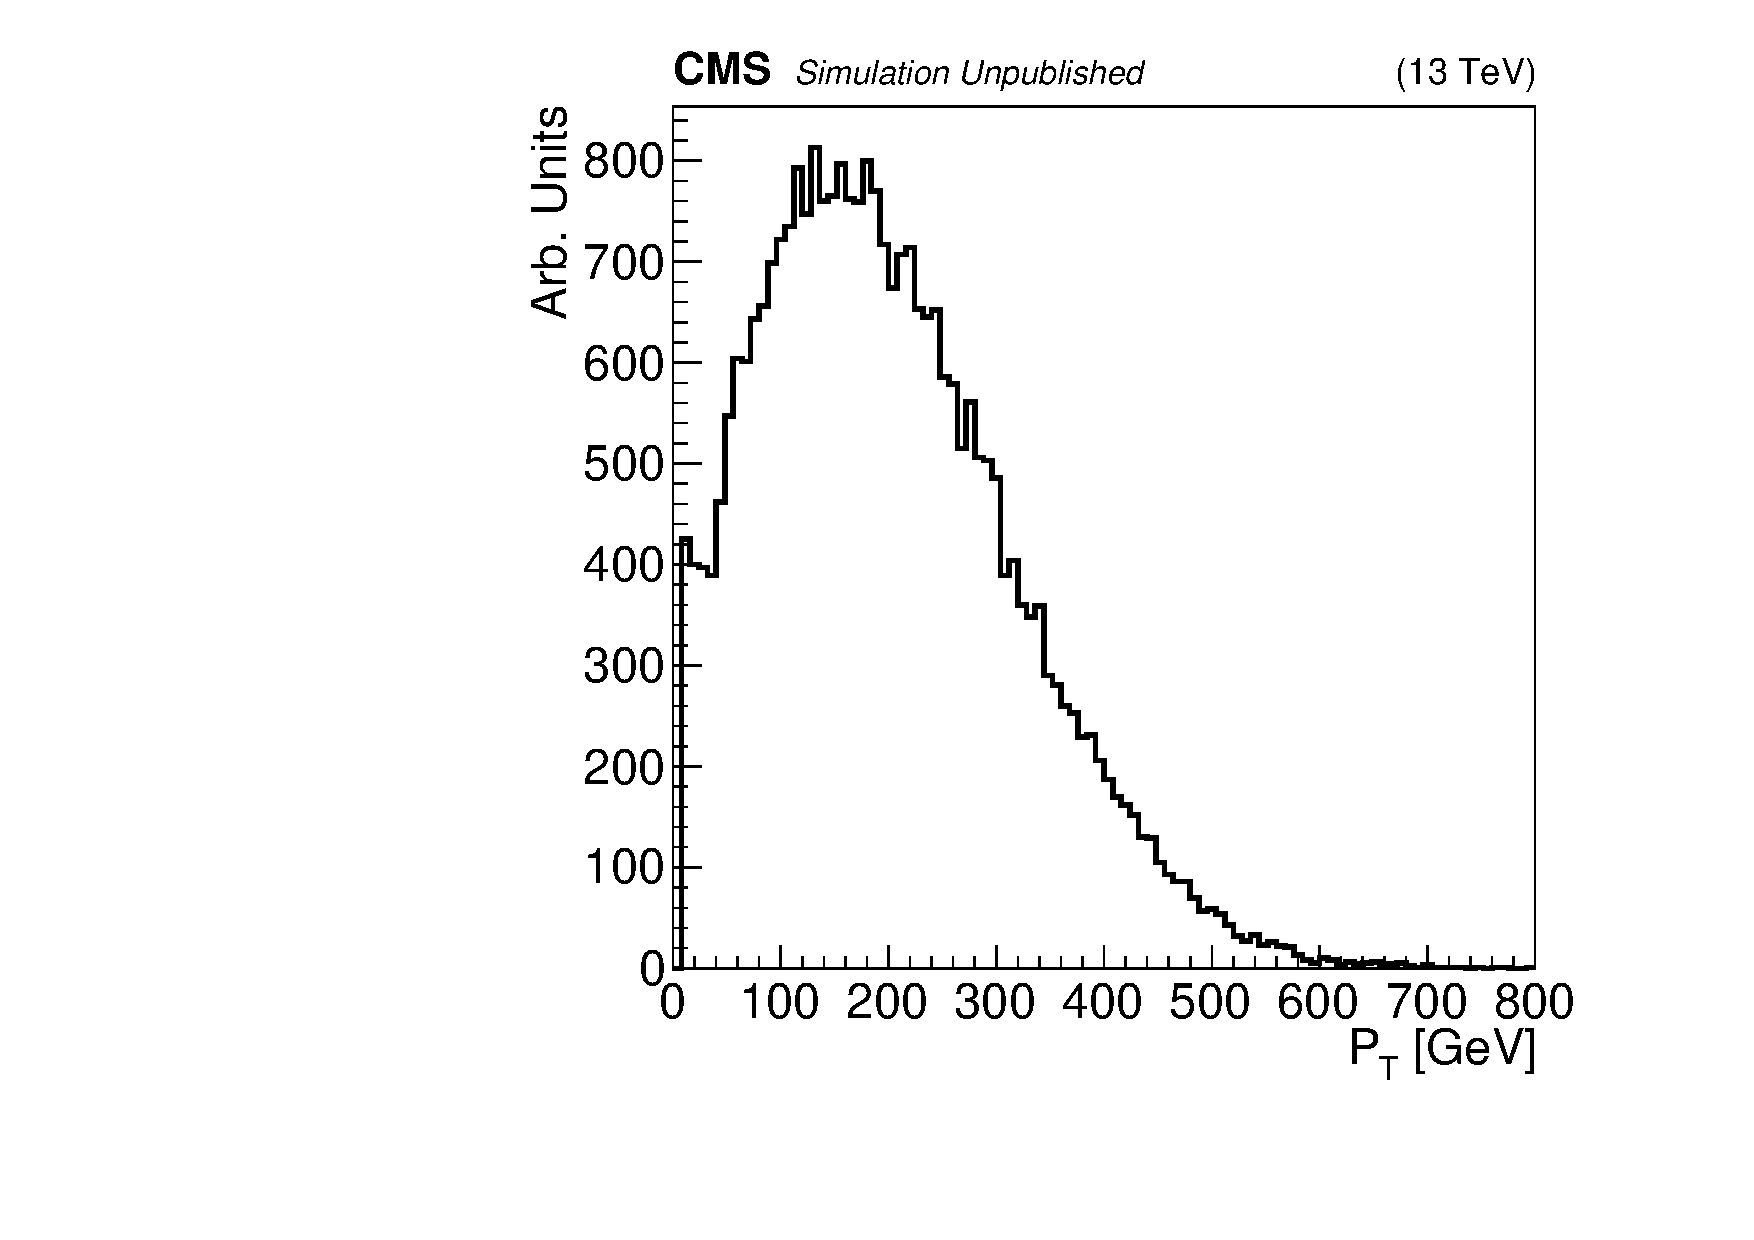
\includegraphics[width=0.45\textwidth]{figures/ptMatchedRecoJetTwo_mwr2200_mnu1100.pdf}
	}
	\label{fig:wrJetPts}
	\caption{The $\pt$ distributions of the reconstructed jets produced by the \nul decay are shown for 
		simulated $\WR \rightarrow eejj$ events with $\mWR = 2.2 \TeV$ and $\mnul = 1.1 \TeV$.}
\end{figure}

\begin{figure}[btp]
	\centering
	\subfigure{
		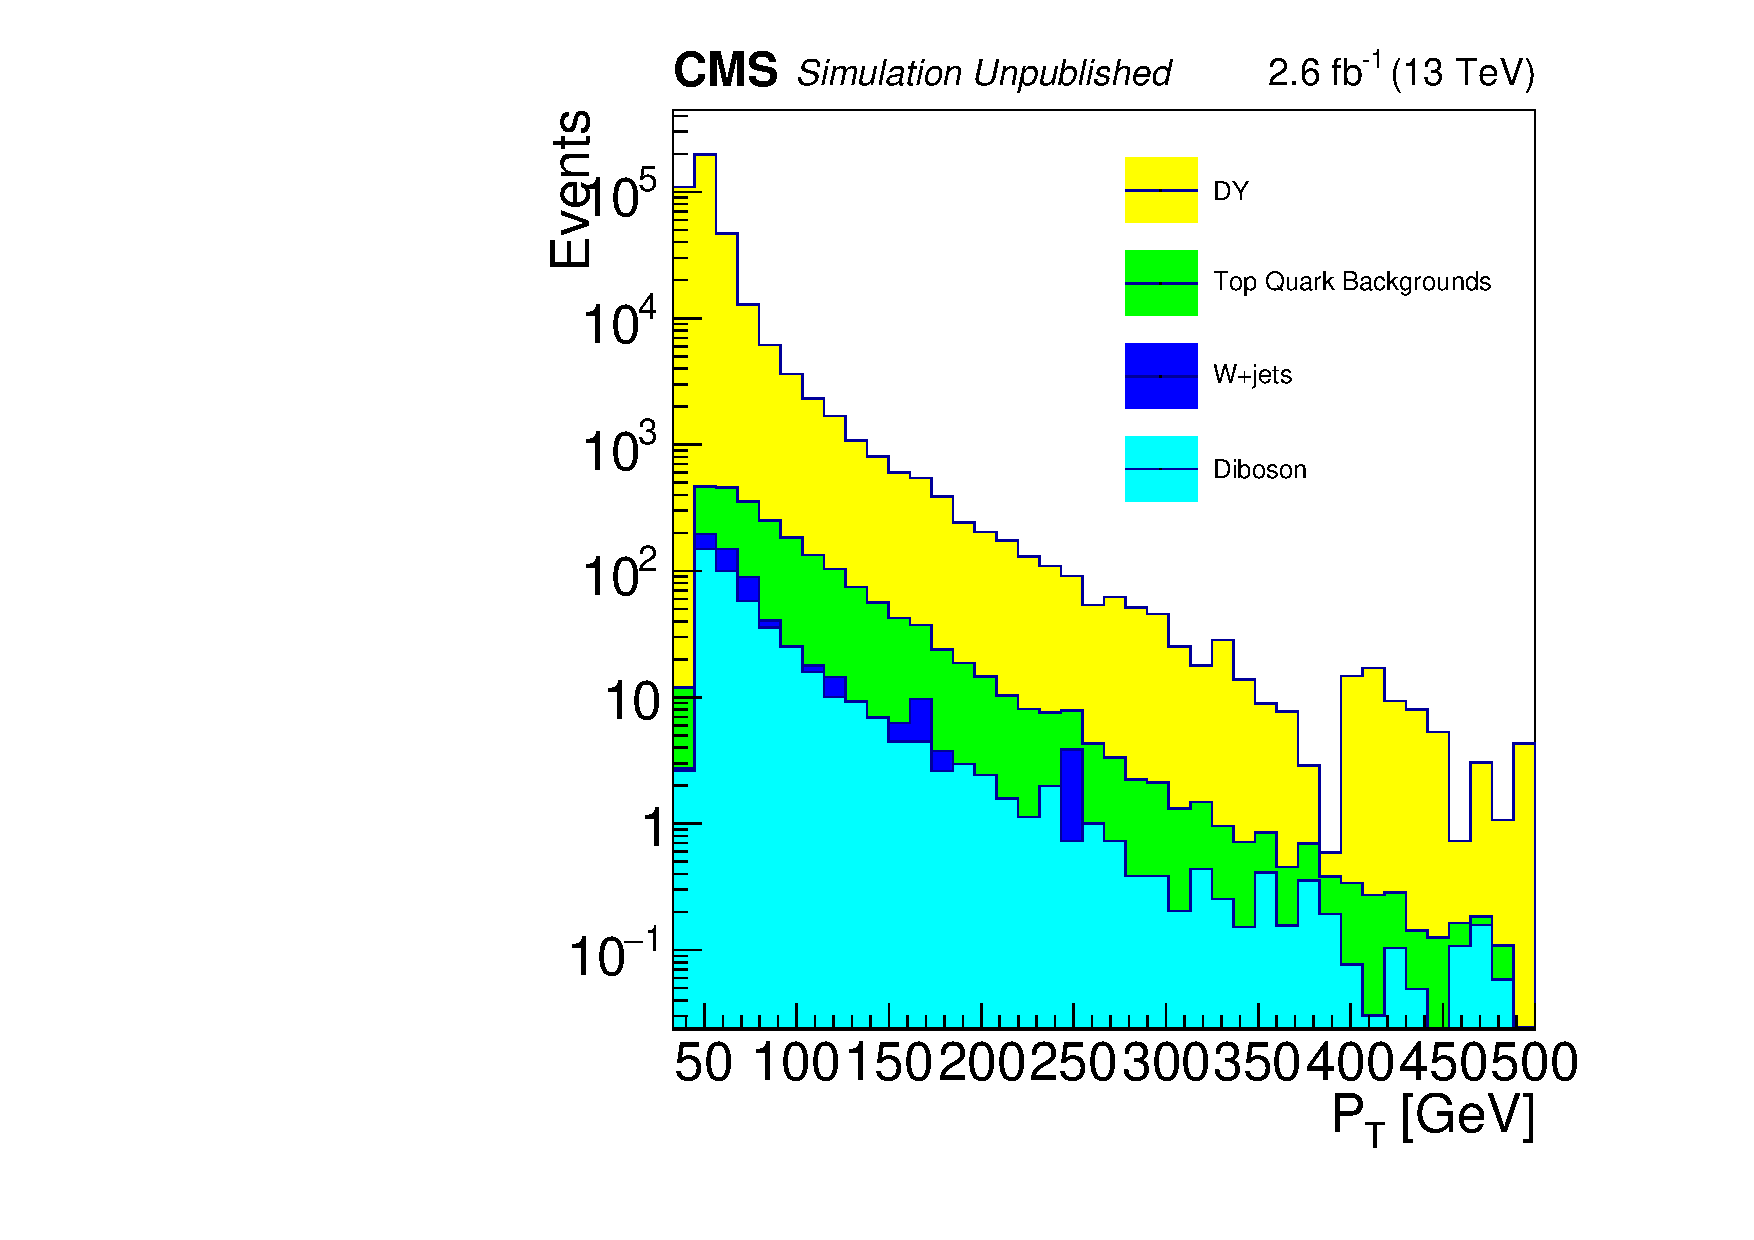
\includegraphics[width=0.45\textwidth]{figures/l1_pt_LooseSelection_TwoLeptsAndJets_EEChannelBkgndMC_log.pdf}
	}
	\subfigure{
		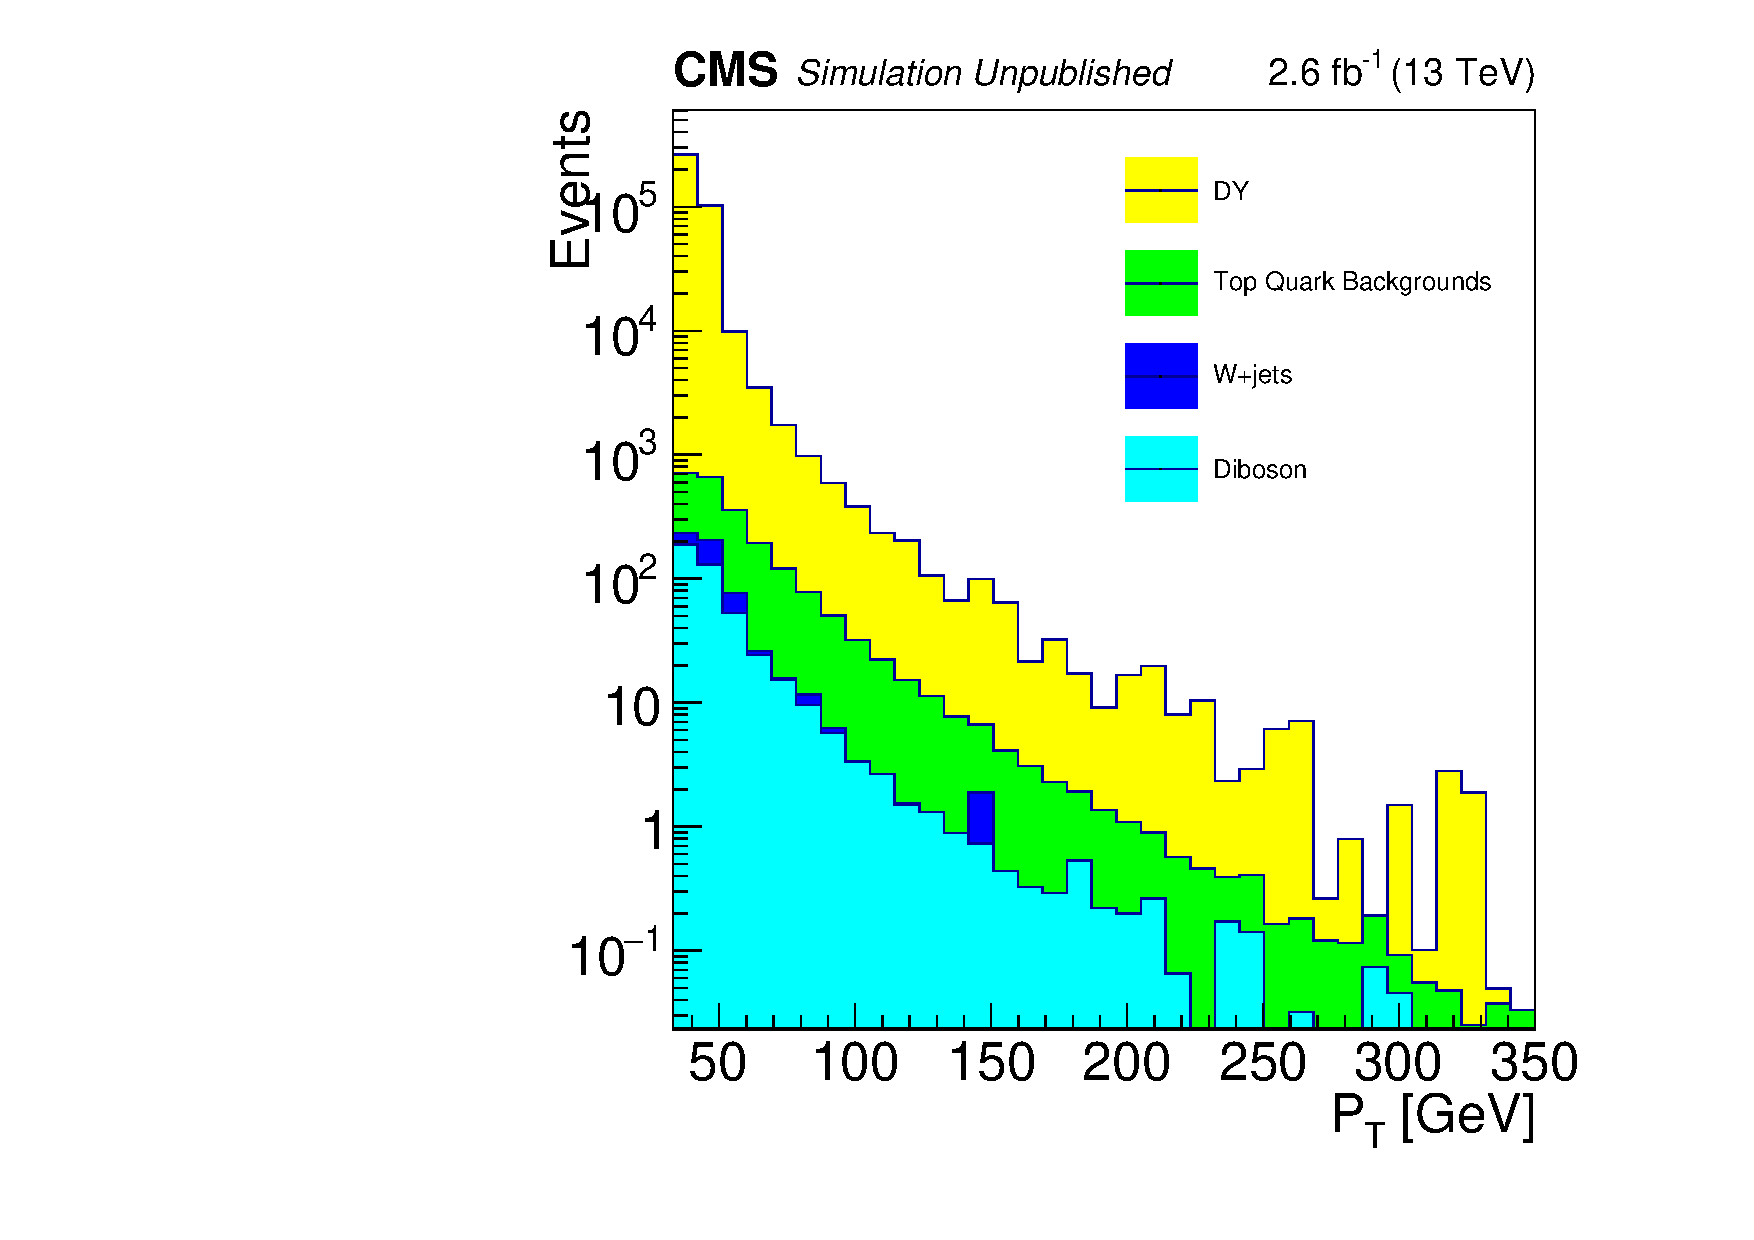
\includegraphics[width=0.45\textwidth]{figures/l2_pt_LooseSelection_TwoLeptsAndJets_EEChannelBkgndMC_log.pdf}
	}
	\label{fig:bkgLeptonPts}
	\caption{The $\pt$ distribution of the leading (subleading) electron reconstructed with $|\eta| < 2.4$ in simulated ST background events 
		with two reconstructed jets is shown on the top (bottom).  Both electrons are required to have $\pt > 33$ $\GeV$.}
\end{figure}

\begin{figure}[btp]
	\centering
	\subfigure{
		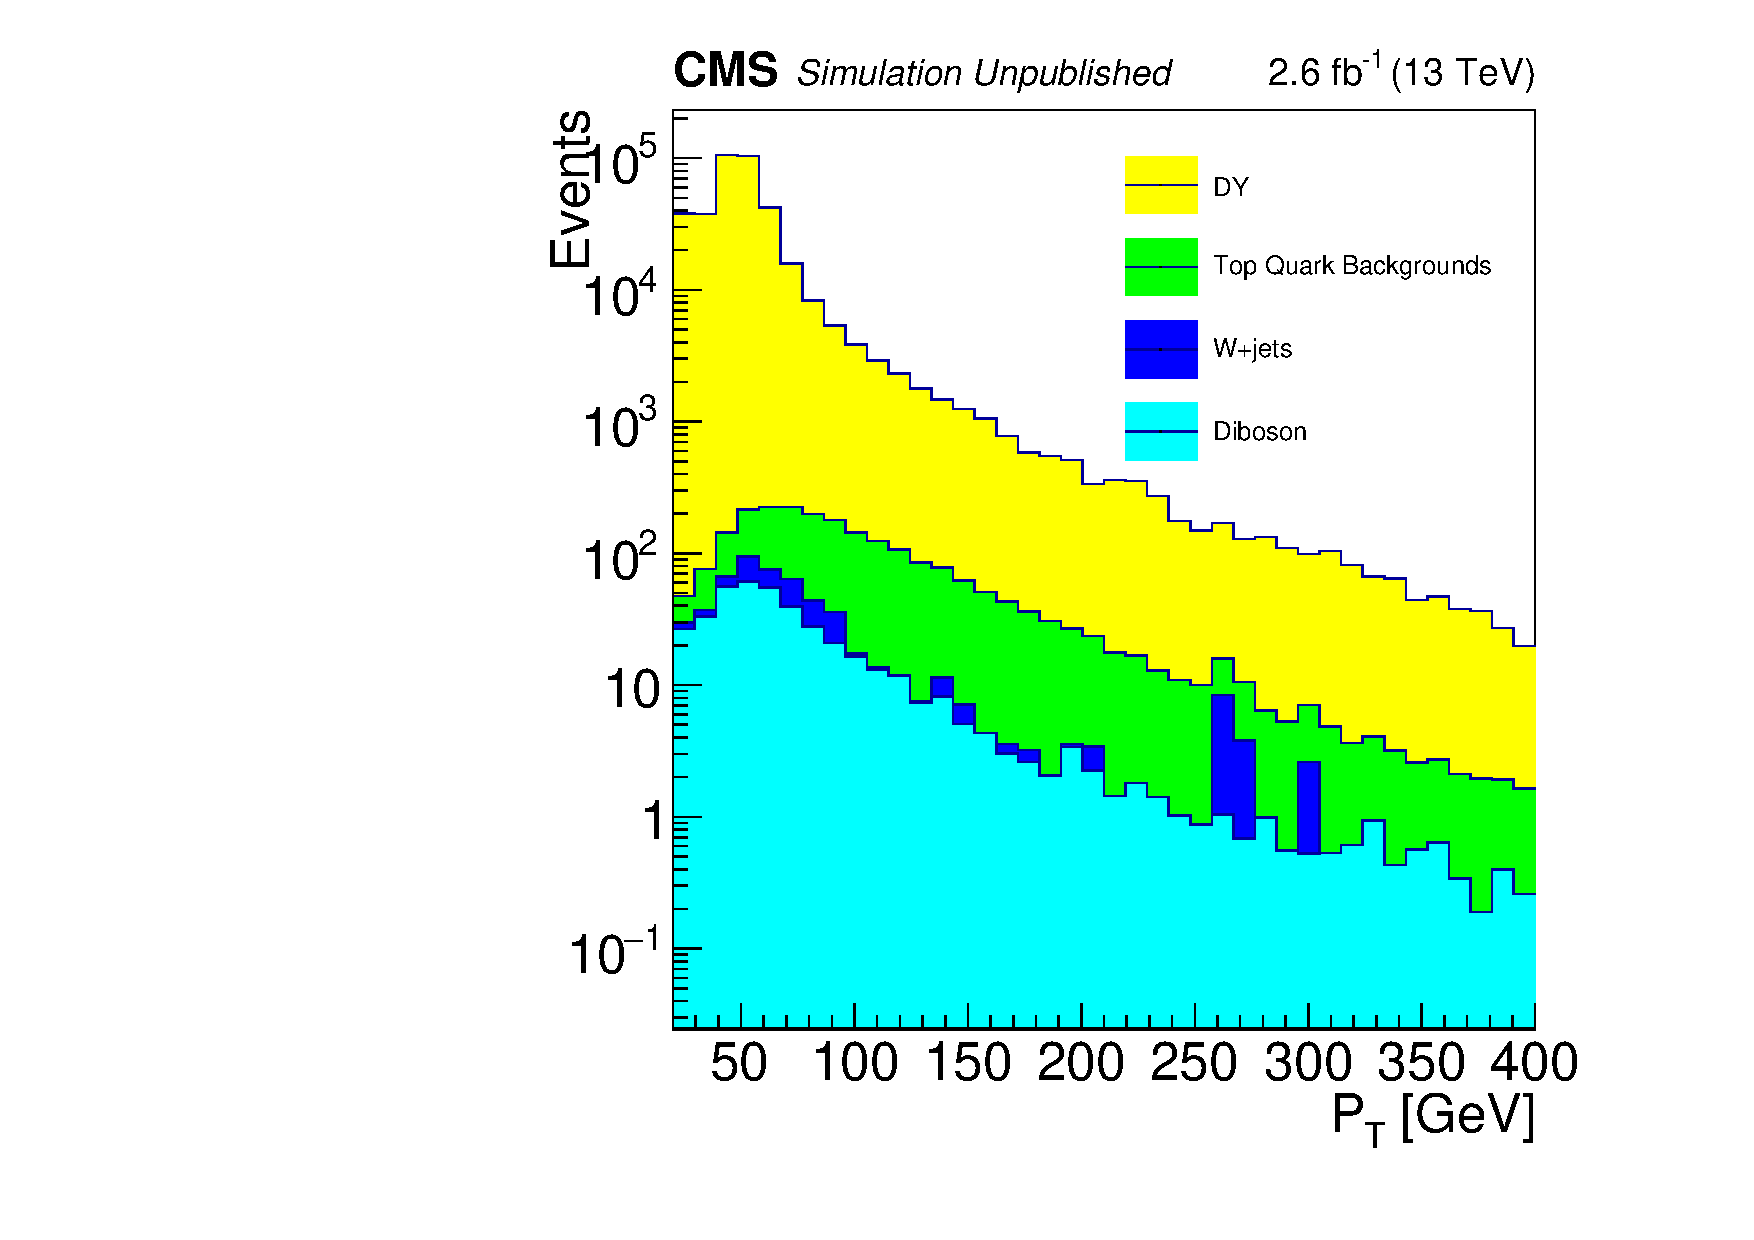
\includegraphics[width=0.45\textwidth]{figures/j1_pt_LooseSelection_TwoLeptsAndJets_EEChannelBkgndMC_log.pdf}
	}
	\subfigure{
		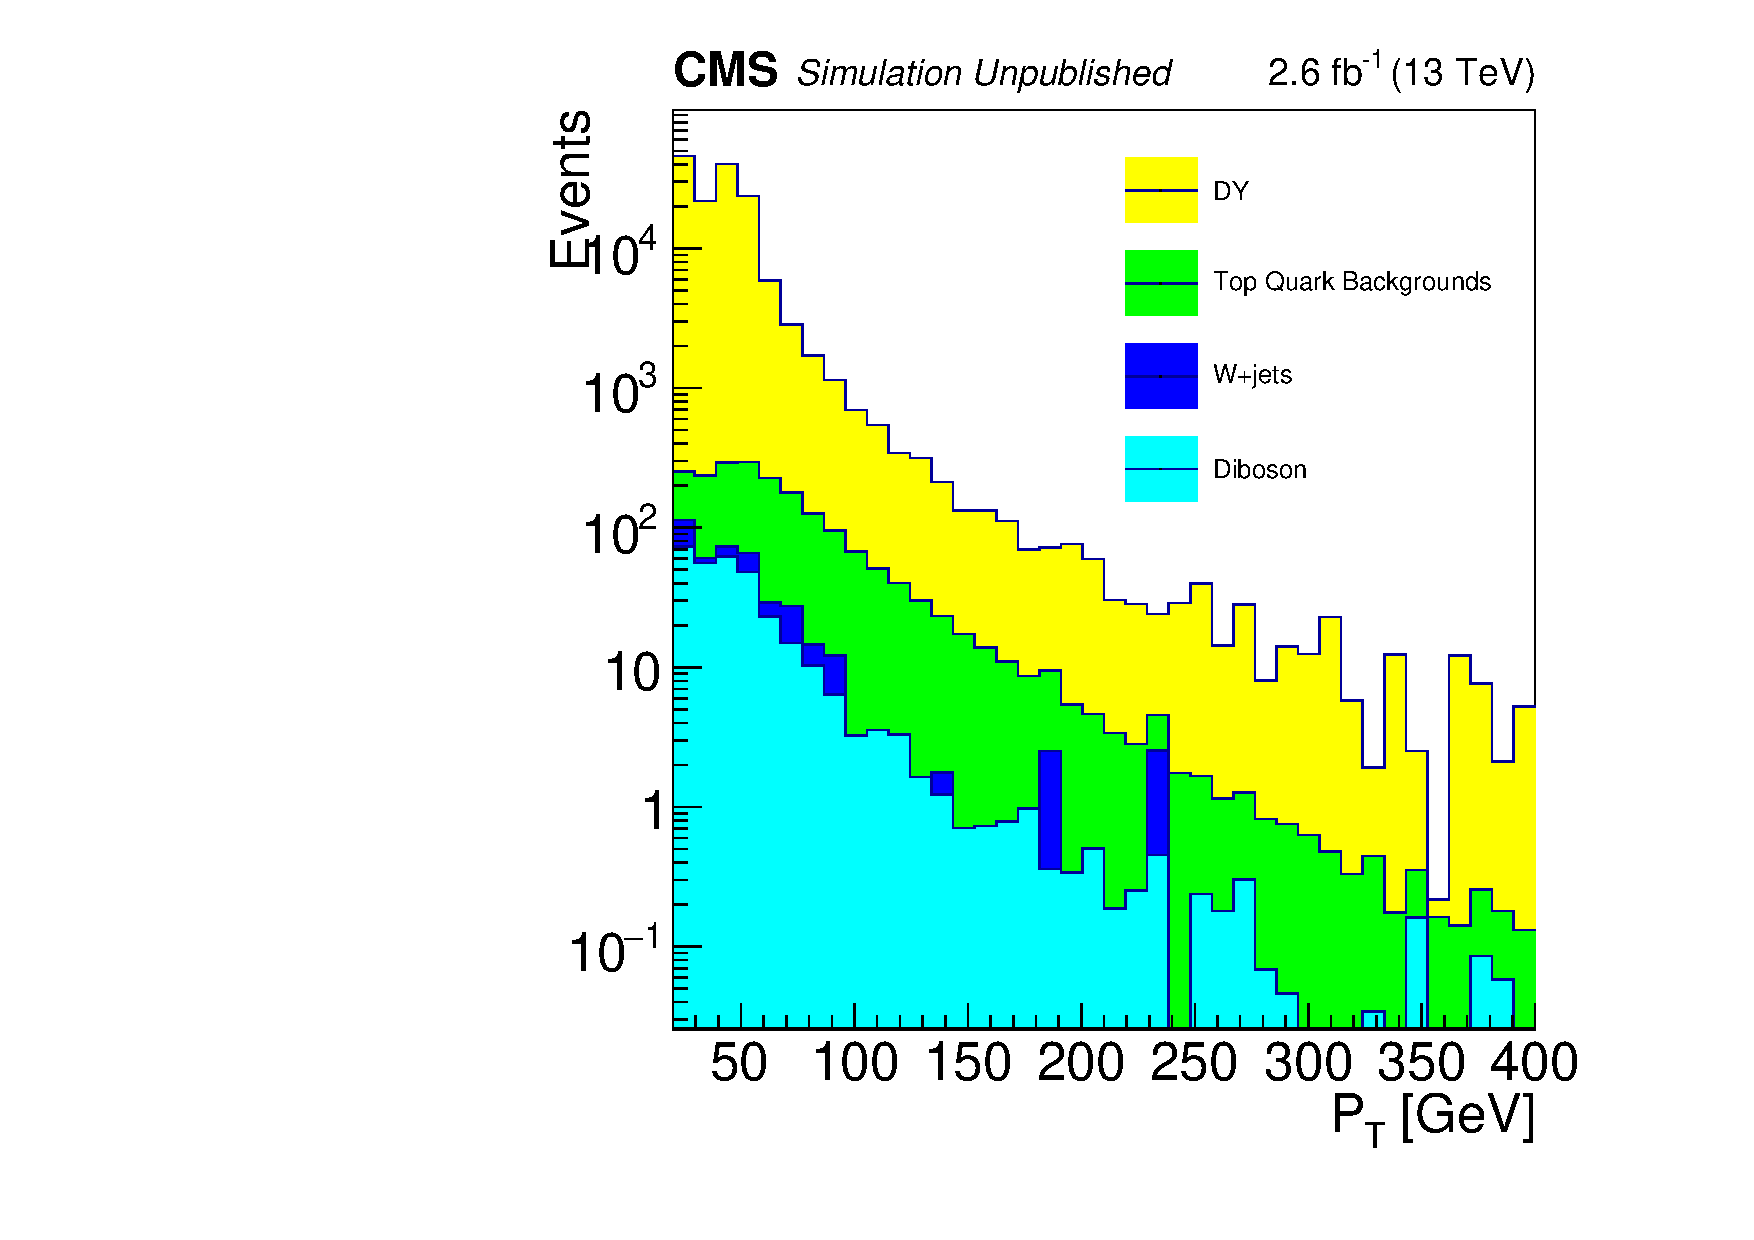
\includegraphics[width=0.45\textwidth]{figures/j2_pt_LooseSelection_TwoLeptsAndJets_EEChannelBkgndMC_log.pdf}
	}
	\label{fig:bkgJetPts}
	\caption{The $\pt$ distribution of the leading (subleading) jet reconstructed with $|\eta| < 2.4$ in simulated ST background events with 
		two reconstructed electrons is shown on the top (bottom).  Both electrons are required to have $\pt > 33$ $\GeV$.}
\end{figure}

%\begin{table}[h]
%	\caption{The fraction of simulated $\WR \rightarrow eejj$ events with dilepton mass $\Mll > 200$ \GeV. ($\mnul = \frac{1}{2}\mWR$)}
%	\label{tab:wrMll}
%	\centering
%	\begin{tabular}{c|c}
%		\mWR (\TeV) & Fraction of events with high \Mll (\%) \\  \hline
%		1.0 &  88.  \\
%		2.0 &  98.  \\
%		3.0 &  99.  \\ \hline
%	\end{tabular}
%\end{table}

%\begin{figure}[btp]
%	\centering
%	
\includegraphics[width=0.65\textwidth]{figures/missingImage.png}
%	\label{fig:wrSigMll}
%	\caption{The dilepton mass $\Mll$ distribution for $\WR \rightarrow \mu\mu jj$ events with 
%	$\mWR = 2.0 \TeV$ and $\mnul = 1.0 \TeV$.}
%\end{figure}

%\begin{figure}[btp]
%	\centering
%	\subfigure{
%		
\includegraphics[width=0.65\textwidth]{figures/missingImage.png}
%	}
%	\subfigure{
%		
\includegraphics[width=0.65\textwidth]{figures/missingImage.png}
%	}
%	\label{fig:wrLeadLeptJetSeparation}
%	\caption{The $\Delta R(\ell,j)$ separation between the leading reconstructed muon and leading (sub-leading) reconstructed jet 
%		is shown on the top (bottom) for $\WR \rightarrow eejj$ events with $\mWR = 2.0 \TeV$ and $\mnul = 1.0 \TeV$.}
%\end{figure}
%
%\begin{figure}[btp]
%	\centering
%	\subfigure{
%		
\includegraphics[width=0.65\textwidth]{figures/missingImage.png}
%	}
%	\subfigure{
%		
\includegraphics[width=0.65\textwidth]{figures/missingImage.png}
%	}
%	\label{fig:wrSubleadLeptJetSeparation}
%	\caption{The $\Delta R(\ell,j)$ separation between the sub-leading reconstructed muon and leading (sub-leading) reconstructed jet 
%		is shown on the top (bottom) for $\WR \rightarrow eejj$ events with $\mWR = 2.0 \TeV$ and $\mnul = 1.0 \TeV$.}
%\end{figure}


\section{Online Event Selection}
\label{sec:triggers}
Evidence of a \WR and \nul was searched for as an excess of events in data relative to predicted backgrounds.  During collisions 
data events in the $ee$-channel were selected using a double electron HLT algorithm, and events in the $\mu\mu$-channel were 
selected using a single muon HLT algorithm.

In the $ee$-channel, events were first selected by Level-1 triggers that required one 5 $\times$ 5 crystal region (one trigger tower, 
or TT) with $\Et > 40 \GeV$, or two TTs: one with $\Et > 22$ $\GeV$, the other with $\Et > 10$ $\GeV$.  Events that passed the 
Level-1 selection were reconstructed offline if they passed the following double electron HLT selections:

\begin{itemize}
	\item Two TTs separated by $\Delta R > 0.1$ were detected with $\Et > 33$ $\GeV$.
	\item In each TT:
	\begin{itemize}
		\item The ratio of hadronic energy in the HCAL tower behind the TT to the TT energy was $< 0.15$ in the barrel, and $< 0.1$ in the endcap.
		\item Ninety percent of the TT energy was measured in an $(\eta, \phi)$ region that was two crystals wide in $\eta$.
		\item If the TT was in the barrel, a reconstructed track with hits in at least two pixel tracker layers extrapolated to the TT 
			centroid along the beam axis within $2.3$ cm, and extrapolated to the TT centroid in $(\eta, \phi)$ within the $(\eta, \phi)$ 
			area of one ECAL crystal.
	\end{itemize}
\end{itemize}

In the $\mu\mu$-channel, events were first selected by a Level-1 trigger that required a track in at least one muon DT or 
CSC detector with $\pt > 16$ $\GeV$.  Events that passed the Level-1 selection were reconstructed offline if they 
passed the following single muon HLT selections:

%RESUME HERE
\begin{itemize}
	\item A track reconstructed in the silicon tracker with $\pt > 50$ $\GeV$ and $|\eta| < 2.4$ was geometrically matched to 
		the muon detector hits that passed the L1 trigger.  Considering this set of muon detector hits and the matching reconstructed 
		track:
	\begin{itemize}
		\item A curve representing the muon trajectory through CMS was fitted to the reconstructed track and at least 
			one muon detector hit with $\chi^{2}/nDOF < 20$.
		\item In the plane perpendicular to the beam axis, the distance between the reconstructed track origin and its 
			reconstructed vertex was $< 1$ mm.
	\end{itemize}
\end{itemize}

Simulated events used in either channel were required to pass the appropriate trigger.


\section{Offline Muon Selection}
\label{sec:muonSelection}
Muon kinematic and identification (ID) selections were applied to select muons consistent 
with those expected from \WR decays.  Each event was required to have two muons reconstructed with 
$\pt > 53$ $\GeV$ and $|\eta| < 2.4$, and at least one with $\pt > 60$ $\GeV$.  
Reducing the lower $\pt$ selection was explored, but was found to increase ST backgrounds without a corresponding increase 
in \WR signal, as shown in Table \ref{tab:lowerMuonPtCuts}.  Muons passing kinematic requirements were selected with the 
following ID selections:

\begin{itemize}
	\item The muon track reconstructed in the silicon tracker:
	\begin{itemize}
		\item The track was reconstructed from at least 1 hit in the silicon pixel detector, and at least 
			5 hits in the entire tracker.
		\item Within a cone of radius $\Delta R = 0.3$ centered on the track, the $\sum \pt$ of all other 
			reconstructed tracks was low compared to the muon $\pt$, $\frac{\sum \pt}{muon \pt} < 0.1$.
	\end{itemize}
	\item The muon was detected in at least 2 muon chambers.
	\item The fitted track representing the estimated muon trajectory through all of CMS originated at a 
		point that was within 2 (5) mm of the muon's reconstructed vertex in the $x-y$ plane ($z$ axis). 
	\item The muon momentum measurement included at least one muon chamber hit.
	\item The error on the muon momentum measurement, $\sigma(\pt)$, was less than 30\% of the muon $\pt$, 
		$\sigma(\pt)/\pt < 0.3$.
\end{itemize}

\begin{table}[h]
	\caption{Signal (S) over background (B) sensitivity, represented by S/$\sqrt{B}$, for different $\mu$ $\pt$ 
	selections.  The background is estimated from simulated \DY and t$\bar{t}$, and the signal is estimated 
	from simulated $\WR \rightarrow \mu\mu jj$ with $\mWR = 2.2 \TeV$ and $\mnul = 1.1 \TeV$.}
	\label{tab:lowerMuonPtCuts}
	\centering
	\begin{tabular}{c|c}
		$\mu$ $\pt$ threshold ($\GeV$) & S/$\sqrt{B}$ \\  \hline
		40 &  11.9  \\
		53 &  12.6  \\ \hline
	\end{tabular}
\end{table}

If an event contained more than two muons passing all kinematic and ID selections, the two highest $\pt$ muons 
were selected.

The efficiencies of muon reconstruction, trigger and ID selections differed between simulations and data, and 
the differences were corrected by applying multiplicative weights to simulated events.  Trigger 
and reconstruction+ID weights were calculated as functions of the charge and kinematic variables of selected 
muons.  The trigger weight, between 0.95 (5\% decrease) and 1.04 (4\% increase), was applied once to every 
event, and the reconstruction+ID weight, between 1.0 and 0.985 (1.5\% decrease), was applied twice to 
every event.


\section{Offline Electron Selection}
\label{sec:electronSelection}
Electron kinematic and ID selections were applied to select electrons 
consistent with those expected from \WR decays.  Each event was required to have two electrons reconstructed 
with $\Et > 53$ $\GeV$ and $|\eta| < 2.4$, and at least one with $\Et > 60$ $\GeV$.  
Electrons passing kinematic requirements were selected with the following ID selections:

\begin{itemize}
	\item Electrons were ignored if they were reconstructed in the dead zone separating the ECAL barrel and 
		endcap detectors, $1.44 < |\eta| < 1.57$.
	\item For endcap electrons, at least 90\% of the SC energy was measured in a region 2 crystals wide in $\eta$.
	\item For barrel electrons, at least 94\% (83\%) of the SC energy was measured in a region 2 (1) crystals wide 
		in $\eta$.
	\item The ratio of hadronic energy in the HCAL tower behind the SC to the SC energy $E_{SC}$ was $< 0.05 + 1/E_{SC}$ 
		in the barrel, and $< 0.05 + 5/E_{SC}$ in the endcap.
	\item In a cone of radius $\Delta R =$ 0.3 centered on the electron's $(\eta, \phi)$ position:
	\begin{itemize}
		\item The $\sum \pt$ of all tracks excluding the electron track was low, $\sum \pt < 5$ $\GeV$.
		\item The total calorimeter energy $E_{ECAL + HCAL}$ in the cone not associated with the electron was low, 
			$E_{ECAL + HCAL} < 2 + 0.03\alpha + 0.28\rho$.  $\rho$ was the neutral hadron energy per unit $\eta,\phi$ area, 
			$\alpha$ in the barrel was the electron $\Et$, and $\alpha$ in the endcap was the electron $\Et$ minus 50 $\GeV$.
	\end{itemize}
	\item The electron's track extrapolated to the $(\eta, \phi)$ position of its SC seed crystal within 1 crystal width in 
		$\eta$, and within $\sim$3 crystal widths in $\phi$.
	\item The electron track missed 1 or fewer layers in the silicon pixel or inner silicon strip detectors.
	\item The electron track origin and its reconstructed vertex were separated by a small distance in the $x-y$ plane, 
		$\Delta_{xy} < 0.2$ mm in the tracker barrel, and $\Delta_{xy} < 0.5$ mm in the tracker endcap.
\end{itemize}

If an event contained more than two electrons passing all kinematic and ID selections, the two highest $\Et$ 
electrons were selected.

The efficiencies of electron reconstruction and ID selections\footnote{The electron trigger efficiency was the same 
in data and simulated events within its statistical uncertainty.} differed between simulations and data, and, similar 
to muons, the differences were corrected by applying multiplicative weights to simulated events.  Fixed value reconstruction 
and ID weights were calculated for electrons with $\Et > 53$ $\GeV$, inclusive of $\eta$.  The reconstruction 
weight, 0.982 (1.8\% decrease), and the ID weight, 0.989 (1.1\% decrease), were applied twice to every event.


\section{Offline Jet Selection}
\label{sec:jetSelection}
Jet kinematic and ID selections were applied to select jets consistent 
with those expected from \WR decays.  Each event was required to have two jets reconstructed with $\pt > 40$ $\GeV$ 
and $|\eta| < 2.4$.  Reducing the $\pt$ selection on one jet was explored, but was found to increase ST backgrounds 
without a corresponding increase in \WR signal, as shown in Table \ref{tab:lowerJetPtCuts}.  Jets passing kinematic 
requirements were selected with the following ID selections:

\begin{itemize}
	\item The jet had at least 2 constituents.
	\item The jet had at least 1 charged hadron constituent.
	\item More than 0\% of the total jet energy came from charged hadrons.
	\item Less than 90\% of the total jet energy came from neutral hadrons.
	\item Less than 90\% of the total jet energy came from photons.
	\item Less than 99\% of the total jet energy came from electrons.
\end{itemize}

\begin{table}[h]
	\caption{Signal (S) over background (B) sensitivity, represented by S/$\sqrt{B}$, for different $\pt$ 
	selections on one jet.  The background is estimated from simulated \DY and t$\bar{t}$, and the 
	signal is estimated from simulated $\WR \rightarrow \mu\mu jj$ with $\mWR = 2.2 \TeV$ and $\mnul = 1.1 \TeV$.}
	\label{tab:lowerJetPtCuts}
	\centering
	\begin{tabular}{c|c}
		jet $\pt$ threshold ($\GeV$) & S/$\sqrt{B}$ \\  \hline
		30 &  12.1  \\
		40 &  12.6  \\ \hline
	\end{tabular}
\end{table}

If an event contained more than two jets passing all kinematic and ID selections, the two highest $\pt$ jets were selected.

The efficiencies of jet reconstruction and ID selections were the same in data and simulated events within uncertainties, so 
no additional corrective weights were needed.


\section{\WR Candidate Selection}
\label{sec:wrCandSelection}
In each event passing trigger, lepton, and jet selections, a \WR candidate was built from selected leptons and jets, and 
a candidate was selected using the following kinematic requirements:

\begin{itemize}
	\item Each selected lepton was separated from the other selected lepton and both jets by $\Delta R > 0.4$.
	\item The dilepton mass $\Mll$ of the two selected leptons exceeded $\Mll > 200$ $\GeV$.
	\item The invariant mass $\Mlljj$ of the selected leptons and jets exceeded $\Mlljj > 600$ $\GeV$.
\end{itemize}

The total efficiency of trigger, kinematic, and ID selections in \WR signal events varied with \mWR, and exceeded 50\% 
in the $ee$-channel, and 70\% in the $\mu\mu$-channel, as shown in Figure \ref{fig:wrRecoSelectionEff}.  The efficiency was 
lower in the $ee$-channel due to the ECAL gap in electron detection for $1.44 < |\eta| < 1.57$, and tighter ID selections 
applied to electrons relative to muons.

\begin{figure}[h]
	\centering
	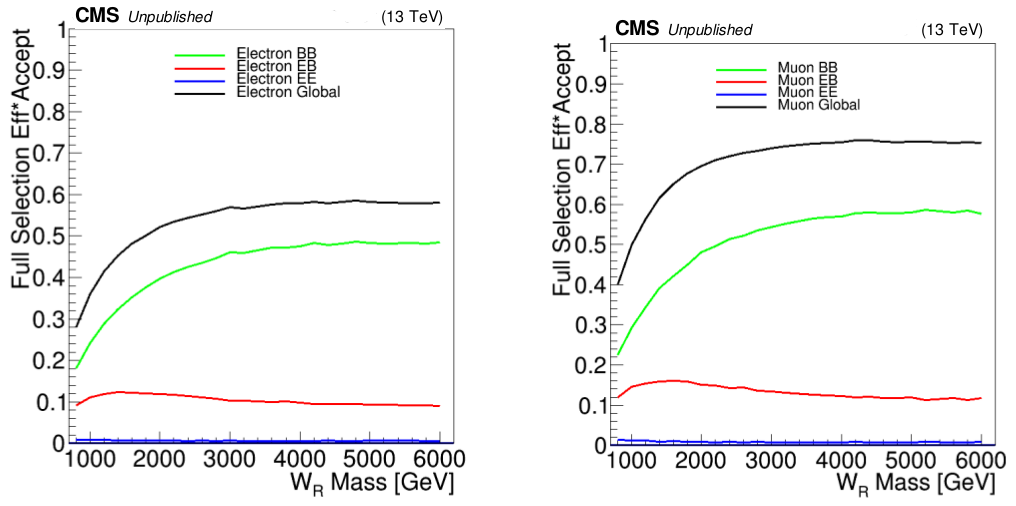
\includegraphics[width=1.0\textwidth]{figures/wrRecoSelectionEfficiency.png}
	\caption{The full selection efficiency in $\WR \rightarrow \ell\ell jj$ events, in the $ee$-channel ($\mu\mu$-channel) 
		on the left (right).  Different curves represent events where both leptons are in the barrel (BB), one was in the 
	endcap (EB), or both were in the endcap (EE).}
	\label{fig:wrRecoSelectionEff}
\end{figure}

After all selections were applied, evidence of a \WR and \nul was searched for as an excess of events over expected backgrounds 
in one kinematic variable distribution.  The existence of a \WR and \nul would create an excess in many kinematic 
variable distributions, like the leading lepton $\pt$ distribution, but for most variables the shape, position, and 
magnitude of the excess is sensitive to the unknown masses \mWR and \mnul.  In addition, in many kinematic variable distributions 
the event selections sculpted expected background events and created a peak away from $0$.  To avoid sculpted 
background distributions and reduce strong sensitivity to \mWR and \mnul, evidence of a \WR and \nul was searched for as an 
excess in the $\Mlljj$ distribution.  There, evidence of a \WR would appear as a peak centered on \mWR 
that can be distinguished from the decaying $\Mlljj$ distribution expected from backgrounds, as shown in Figure 
\ref{fig:mlljjVariableOfMerit}.  Before looking for evidence of a \WR and \nul in data, the $\Mlljj$ distribution expected 
from backgrounds was estimated using data and simulated events in `control` regions where data and simulations were expected 
to agree.

\begin{figure}[h]
	\centering
	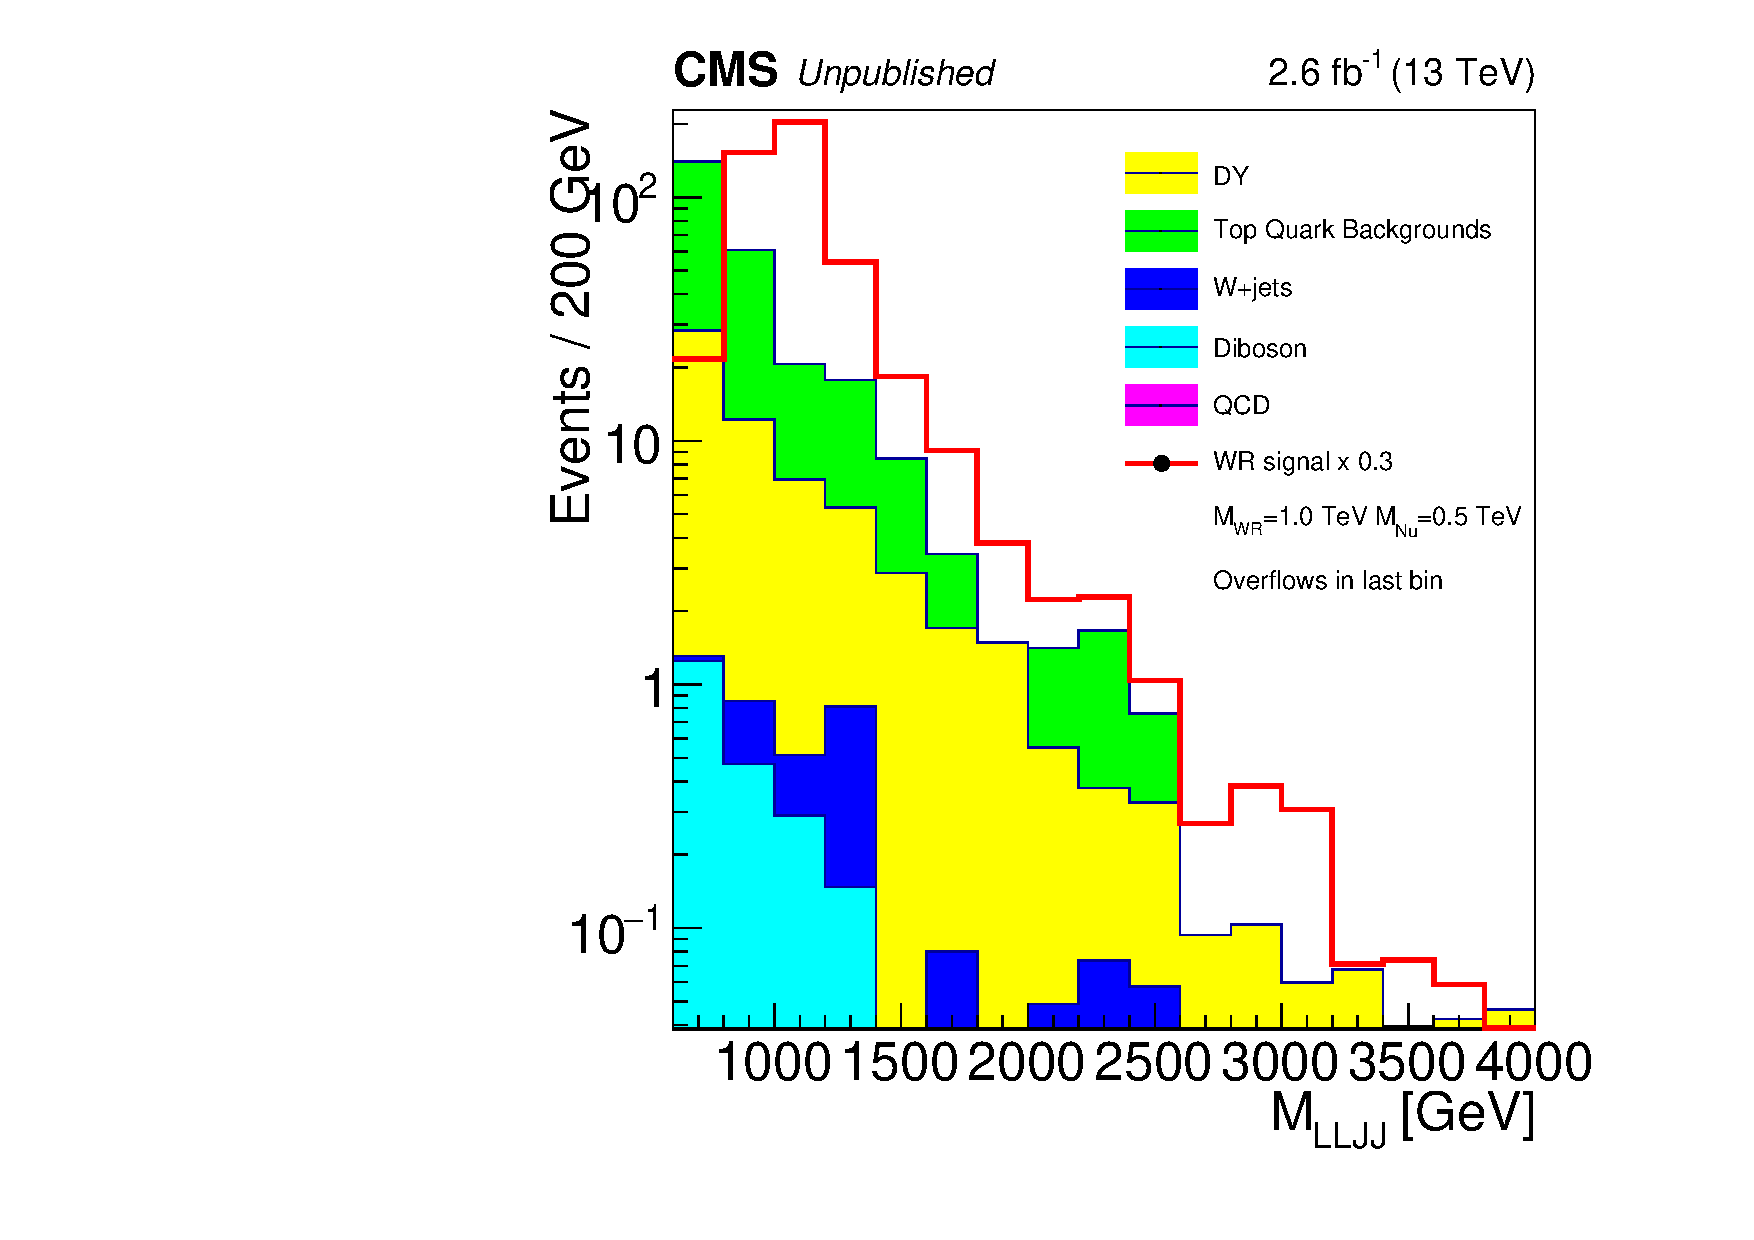
\includegraphics[width=0.7\textwidth]{figures/useOfLLJJMassAsFigureOfMerit.pdf}
	\caption{The $\Mlljj$ distribution from simulations of ST backgrounds and a \WR signal in the $ee$-channel.  
		The \WR signal normalization is reduced by 70\% to better visualize the difference 
	between the signal and expected backgrounds.}
	\label{fig:mlljjVariableOfMerit}
\end{figure}


%%%%%%%%%%%%%%%%%%%%%%%%%%%%%%%%%%%%%%%%%%%%%%%%%%%%%%%%%%%%%%%%%%%%%%%%%%%%%%%%
